\documentclass[a4paper,10pt]{article}
\usepackage[utf8]{inputenc}

% ----  Useful packages % ---- 
\usepackage{amsmath}
\usepackage{graphicx}
\usepackage{amsfonts}
\usepackage{amsthm}
\usepackage{amssymb}
\usepackage{makecell}
% ----  Useful packages % ---- 

\usepackage{wrapfig}
\usepackage{caption}
\usepackage{subcaption}
\usepackage{hyperref}
\hypersetup{
    colorlinks,
    citecolor=black,
    filecolor=black,
    linkcolor=black,
    urlcolor=black
}

\graphicspath{ {./images/} }

% ---- Set page size and margins replace ------
\usepackage[letterpaper,top=2cm,bottom=2cm,left=3cm,right=3cm,marginparwidth=1.75cm]{geometry}
% ---- Set page size and margins replace ------

% ------- NOTA ------
\theoremstyle{remark}
\newtheorem{note}{Note}[subsection]
% ------- NOTA ------

% ------- OSSERVAZIONE ------
\theoremstyle{definition}
\newtheorem{observation}{Osservazione}[subsection]
% ------- OSSERVAZIONE ------

% ------- DEFINIZIONE ------
\theoremstyle{plain}
\newtheorem{definition}{Definizione}[subsection]
% ------- DEFINIZIONE ------

% ------- ESEMPIO ------
\theoremstyle{definition}
\newtheorem{example}{Esempio}[subsection]
% ------- ESEMPIO ------

% ------- DIMOSTRAZIONE ------
\theoremstyle{definition}
\newtheorem{demostration}{Dimotrazione}[subsection]
% ------- DIMOSTRAZIONE ------

% ------- TEOREMA ------
\theoremstyle{definition}
\newtheorem{theorem}{Teorema}[subsection]
% ------- TEOREMA ------

% ------- COROLLARIO ------
\theoremstyle{plain}
\newtheorem{corollaries}{Corollario}[theorem]
% ------- COROLLARIO ------

% ------- PROPOSIZIONE ------
\theoremstyle{plain}
\newtheorem{proposition}{Proposizione}[subsection]
% ------- PROPOSIZIONE ------

% ---- Footer and header ---- 
\usepackage{fancyhdr}
\pagestyle{fancy}
\fancyhf{}
\fancyhead[LE,RO]{A.A 2022-2023}
\fancyhead[RE,LO]{Architettura e Sistemi Operativi}
\fancyfoot[RE,LO]{\rightmark}
\fancyfoot[LE,RO]{\thepage}

\renewcommand{\headrulewidth}{.5pt}
\renewcommand{\footrulewidth}{.5pt}
% ---- Footer and header ---- 

% ----  Language setting ---- 
\usepackage[italian, english]{babel}
% ----  Language setting ---- 

\usepackage{listings}
\usepackage{color}

\definecolor{dkgreen}{rgb}{0,0.6,0}
\definecolor{gray}{rgb}{0.5,0.5,0.5}
\definecolor{mauve}{rgb}{0.58,0,0.82}

\lstset{frame=tb,
  language=C,
  aboveskip=3mm,
  belowskip=3mm,
  showstringspaces=false,
  columns=flexible,
  basicstyle={\small\ttfamily},
  numbers=none,
  numberstyle=\tiny\color{gray},
  keywordstyle=\color{blue},
  commentstyle=\color{dkgreen},
  stringstyle=\color{mauve},
  breaklines=true,
  breakatwhitespace=true,
  tabsize=3
}

\title{\textbf{Architettura e Sistemi Operativi}}
\author{Realizzato da: Giuntoni Matteo}
\date{A.A. 2022-2023}

\begin{document}
\begin{titlepage} %crea l'enviroment
	\begin{figure}[t] %inserisce le figure
		\centering
\includegraphics[width=0.98\textwidth]{marchio_unipi_pant541.png}
	\end{figure}
	\vspace{20mm}
	
	\begin{Large}
		\begin{center}
			\textbf{Dipartimento di Informatica\\ Corso di Laurea Triennale in Informatica\\}
			\vspace{20mm}
			{\LARGE{Corso a Libera Scelta - 6 CFU}}\\
			\vspace{10mm}
			{\huge{\bf Computer Graphics}}\\
		\end{center}
	\end{Large}
	
	
	\vspace{36mm}
	%minipage divide la pagina in due sezioni settabili
	\begin{minipage}[t]{0.47\textwidth}
		{\large{\bf Professore:}\\ \large{Prof. }}
	\end{minipage}
	\hfill
	\begin{minipage}[t]{0.47\textwidth}\raggedleft
		{\large{\bf Autore:}\\ \large{Filippo Ghirardini}}
	\end{minipage}
	
	\vspace{25mm}
	
	\hrulefill
	
	\vspace{5mm}
	
	\centering{\large{\bf Anno Accademico 2023/2024 }}
	
\end{titlepage}

\tableofcontents
\newpage
\maketitle
\begin{center}
    \vspace{-20pt}
    \rule{11cm}{.1pt} 
\end{center}
\section{Introduzione}

\subsection{Insiemi Numerici}
Un insieme di numeri è una raccolta di elementi. Alcuni degli insiemi che verranno utilizzati maggiormente in questo corso sono:
\begin{itemize}
    \item \textbf{N. Naturali} cioè tutti gli interi non negativi: $\mathbb{N}$ = $\{0, 1, 2, 3, 4, ...\}$.
    \item \textbf{N. Interi} cioè tutti gli interi con segno qualsiasi: $\mathbb{Z} = \{..., -3, -2, -1, 0, 1, 2, 3, ...\}$.
    \item \textbf{N. Razionali}, cioè le frazioni: $\mathbb{Q} = \{\frac{p}{q}$ dove p e q $\in \mathbb{Z}$ e $q \neq 0\}$. \\
    Un sottoinsieme sono le \textbf{classi di equivalenza} che sono tutte le frazioni semplificate ai minimi termini. 
    \item \textbf{N. Reali}, che possono essere visti come tutti gli elementi rappresentabili su una retta: $\mathbb{R}$ 
\end{itemize}
\begin{note}
I vari insiemi si contengono fra di loro. ($\mathbb{N} \subset \mathbb{X} \subset \mathbb{Q} \subset \mathbb{R}$) 
\end{note}
\begin{note}
Esistono molti numeri reali che non sono razionali e non si possono scrivere come frazioni. E.g. $\sqrt{2}, \pi, ...$
\end{note}

\subsection{Intervalli}
\begin{definition}[Intervallo]
    Un sottoinsieme $I \subseteq \mathbb{R}$ è un intervallo se $\forall \: x,\:y \in I$ $\mid$ $x < y$ $\wedge$ $\forall z \mid x < z < y$ ho che $z \in I$. [\ref{fig:intervallo}]
\end{definition}
\begin{wrapfigure}{l}{7cm}
	\vspace{-20pt}
	\centering
	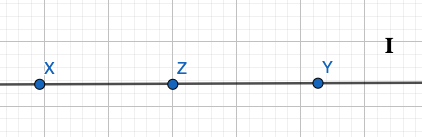
\includegraphics[width=5cm]{Intervallo.png}
	\caption{Tutto il segmento fra x e y deve stare in I}
	\label{fig:intervallo}
\end{wrapfigure}
I è un intervallo se ogni \emph{ogni} punto che prendo tra gli estremi dell'intervallo, questo appartiene all'intervallo stesso.
\\\\\\\\\\
\begin{example}
Esempi di intervalli.\\ \\
Questo caso \textbf{è un intervallo} \hspace{3.2cm} Questo caso \textbf{non è un intervallo} fra A e D.
\begin{figure}[h!]
    \vspace{-10pt}
    \begin{subfigure}{.5\textwidth}
        \hspace{-50pt}
        \centering
        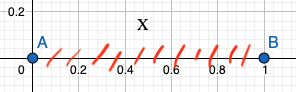
\includegraphics[width=6cm]{Esempio-intervallo-1.png}
        \caption{$A = \{x \in \mathbb{R} \: | \: 0<x<1\}$}
    \end{subfigure}
    \begin{subfigure}{.5\textwidth}
        \centering
        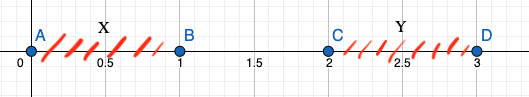
\includegraphics[width=7.5cm]{Esempio-intervallo-2.png}
        \caption{$C = \{x \in \mathbb{R} \: | \: 0<x<1 \: \vee \: z<x<3\}$}
    \end{subfigure}
\end{figure}
\end{example}

\newpage
\subsection{Notazione}
Con $a, b \in \mathbb{R}$ e con $a < b$ è possibile scrivere le notazioni in tabella \ref{tab:notazione-intervalli}.
\begin{table}[h!]
    \centering
    \setlength{\tabcolsep}{7pt}
    \renewcommand{\arraystretch}{2}
    \begin{tabular}{|c|c|c|} \hline
        [a, b] & Intervallo chiuso di estremi a e b & $\{x \in \mathbb{R} \: | \: a \leq x \leq b\}$ \\ \hline
        (a, b) & Intervallo aperto & $\{x \in \mathbb{R} \: | \: a < x < b\}$ \\ \hline
        [a, b) & Intervallo semi aperto a destra & $\{x \in \mathbb{R} \: | \: a \leq x < b\}$ \\ \hline
        (a, b] & Intervallo semi aperto a sinistra & $\{x \in \mathbb{R} \: | \: a < x \leq b\}$ \\ \hline
        [a, $+\infty$) & Semiretta chiusa a sinistra & $\{x \in \mathbb{R} \: | \: a \leq x\}$ \\ \hline
        ($-\infty$, b] & Semiretta chiusa a destra & $\{x \in \mathbb{R} \: | \: x \leq b\}$ \\ \hline
        ($-\infty$, $+\infty$) & Insieme di tutti i numeri $\mathbb{R}$ & $\{x \in \mathbb{R}\}$ \\ \hline
    \end{tabular}
    \caption{Notazione Intervalli}
    \label{tab:notazione-intervalli}
\end{table}
\newpage
% !TeX spellcheck = it_IT
\section{Memory Hierarchy}
I principi fondamentali che andremo a vedere sono legati alle tecnologie con cui vengono costruite le memorie, la gerarchia delle varie tipologie di memorie, le memorie caches ed in fine come andare a misurare e migliorare le performance delle caches.

\subsection{Memory technologies}
Partiamo dicendo che esistono varie tipologie di memorie, che possono essere distinte in primo luogo in \textbf{memorie volatili}, e \textbf{memorie non volatili}. Quelle volatili sono:
\begin{wrapfigure}{r}{5cm}
	\centering
	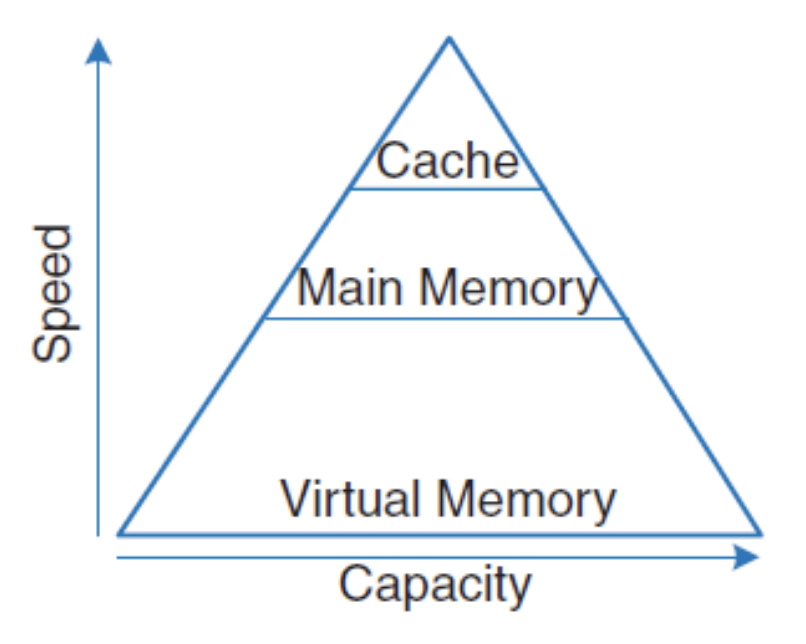
\includegraphics[width=4cm]{images/memory-hierarcgy.png}
	\caption{Gerarchia memoria}
\end{wrapfigure}

\begin{itemize}
    \item Latches, flip-flops, register files (o semplici registri).
    \item SRAM (Static Random-Access Memory).
    \item DRAM (Dynamic Random-Access Memory).
\end{itemize}

\noindent Fra le memorie non volatili invece ci sono:
\begin{itemize}
    \item ROM
    \item NVRAM \footnote{Memoria non volatile nel formato di un banco DRAM che può fornire accesso tramite byte-address.}
    \item Flash memory
    \item Magnetic disks
\end{itemize}

\subsection{Cost vs Capacity vs Access Time}
Un altro confronto interessante da fare fra le memorie è relativamente ai costi, le capacità ed il tempo di accesso.
\begin{center}
	\begin{tabular}{|c|c|c|c|c|}
	\hline
	\textbf{Memoria} &\textbf{Access time (ns)} & Bandwidth (GB/s) & \textbf{Price(\$/GB)} & \textbf{Usage} \\
	\hline
	\textit{SRAM} & $0.5-1$ & $25+$ & $5000$ & Register and caches \\
	\hline
	\textit{DRAM} & $10-50$ & $10$ & $7$ & RAM \\
	\hline
	\textit{Flash} & $20.000$ & $0.5$ & $0.40$ & SSD disks \\
	\hline
	\textit{Magnetic} & $5.000.000$ & $0.75$ & $0.05$ & HDD Disk \\
	\hline
\end{tabular}
\end{center}

\hspace{-15pt}Da questa classificazione possiamo trarre alcune regole generali:
\begin{itemize}
    \item Le memorie di grandi dimensioni sono solitamente lente e economiche.
    \item Le memorie di piccole dimensioni sono più veloci ma anche più costose.
\end{itemize}

\noindent Da qui possiamo capire che nella selezione della memorie va trovato un compromesso fra i parametri visti precedentemente per andare ad avere memorie sufficientemente grandi per contenere i dati richiesti ma allo steso tempo sufficientemente veloci per evitare il \textbf{von Neumann Bottleneck}.

\newpage
\subsection{Von Neumann architecture}
\begin{wrapfigure}{r}{6.5cm}
    \vspace{-25pt}
    \centering
    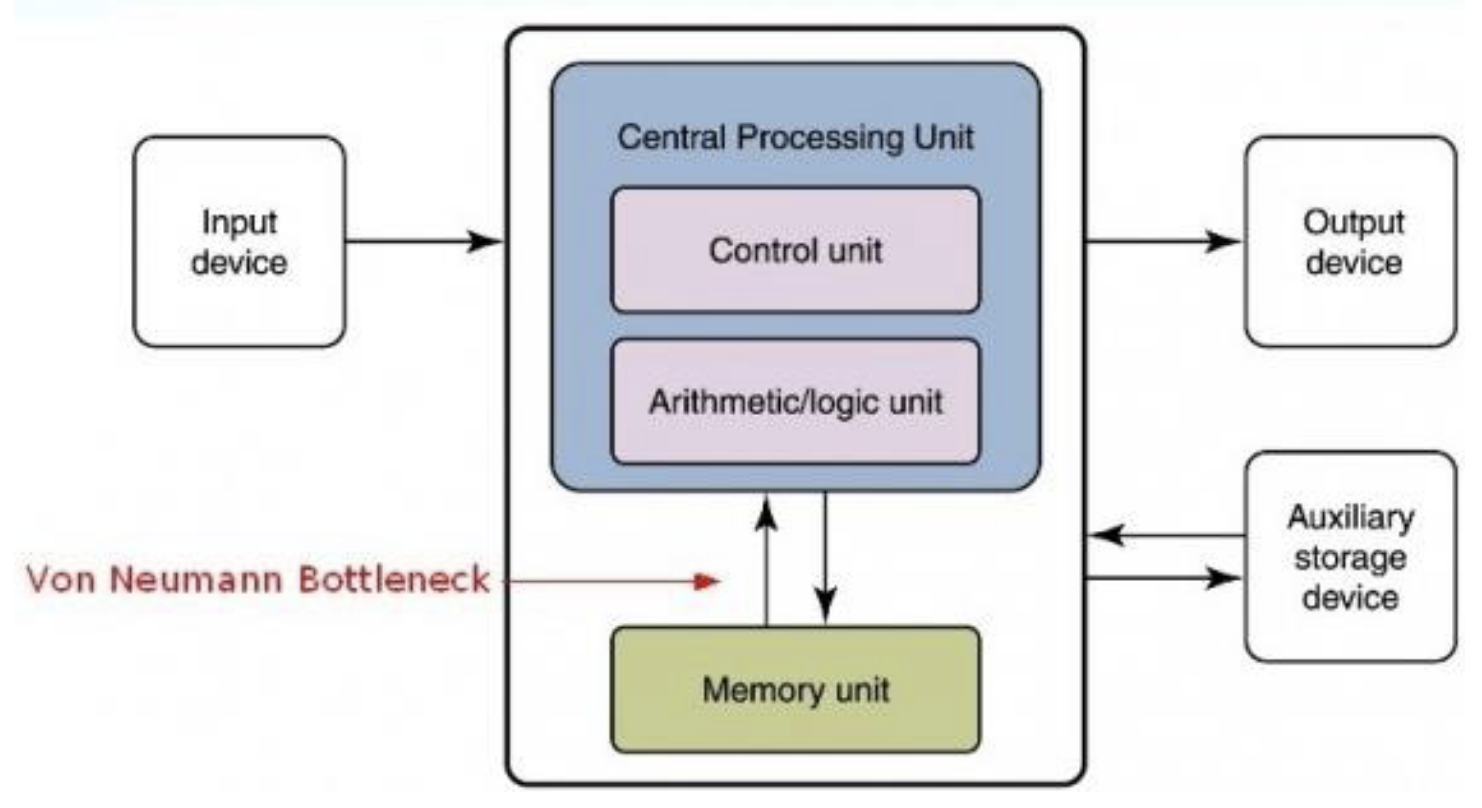
\includegraphics[width=6cm]{images/von-numan.png}
    \caption{Von-Neumann}
\end{wrapfigure}
Le performance dei computer sono limitate nella velocità della CPU dal trasferimento di dati fra le memorie esterne dall'unità di calcolo.\\
Per mitigare questo problema inseriamo memorie più piccole e veloci vicino al processore, mentre più ci si allontana più si avranno memorie grosse e lente. In questo modo facciamo lavorare il processore alla velocità della memoria più vicina.\\\\

\begin{wrapfigure}{l}{6.5cm}
    \vspace{-10pt}
    \centering
    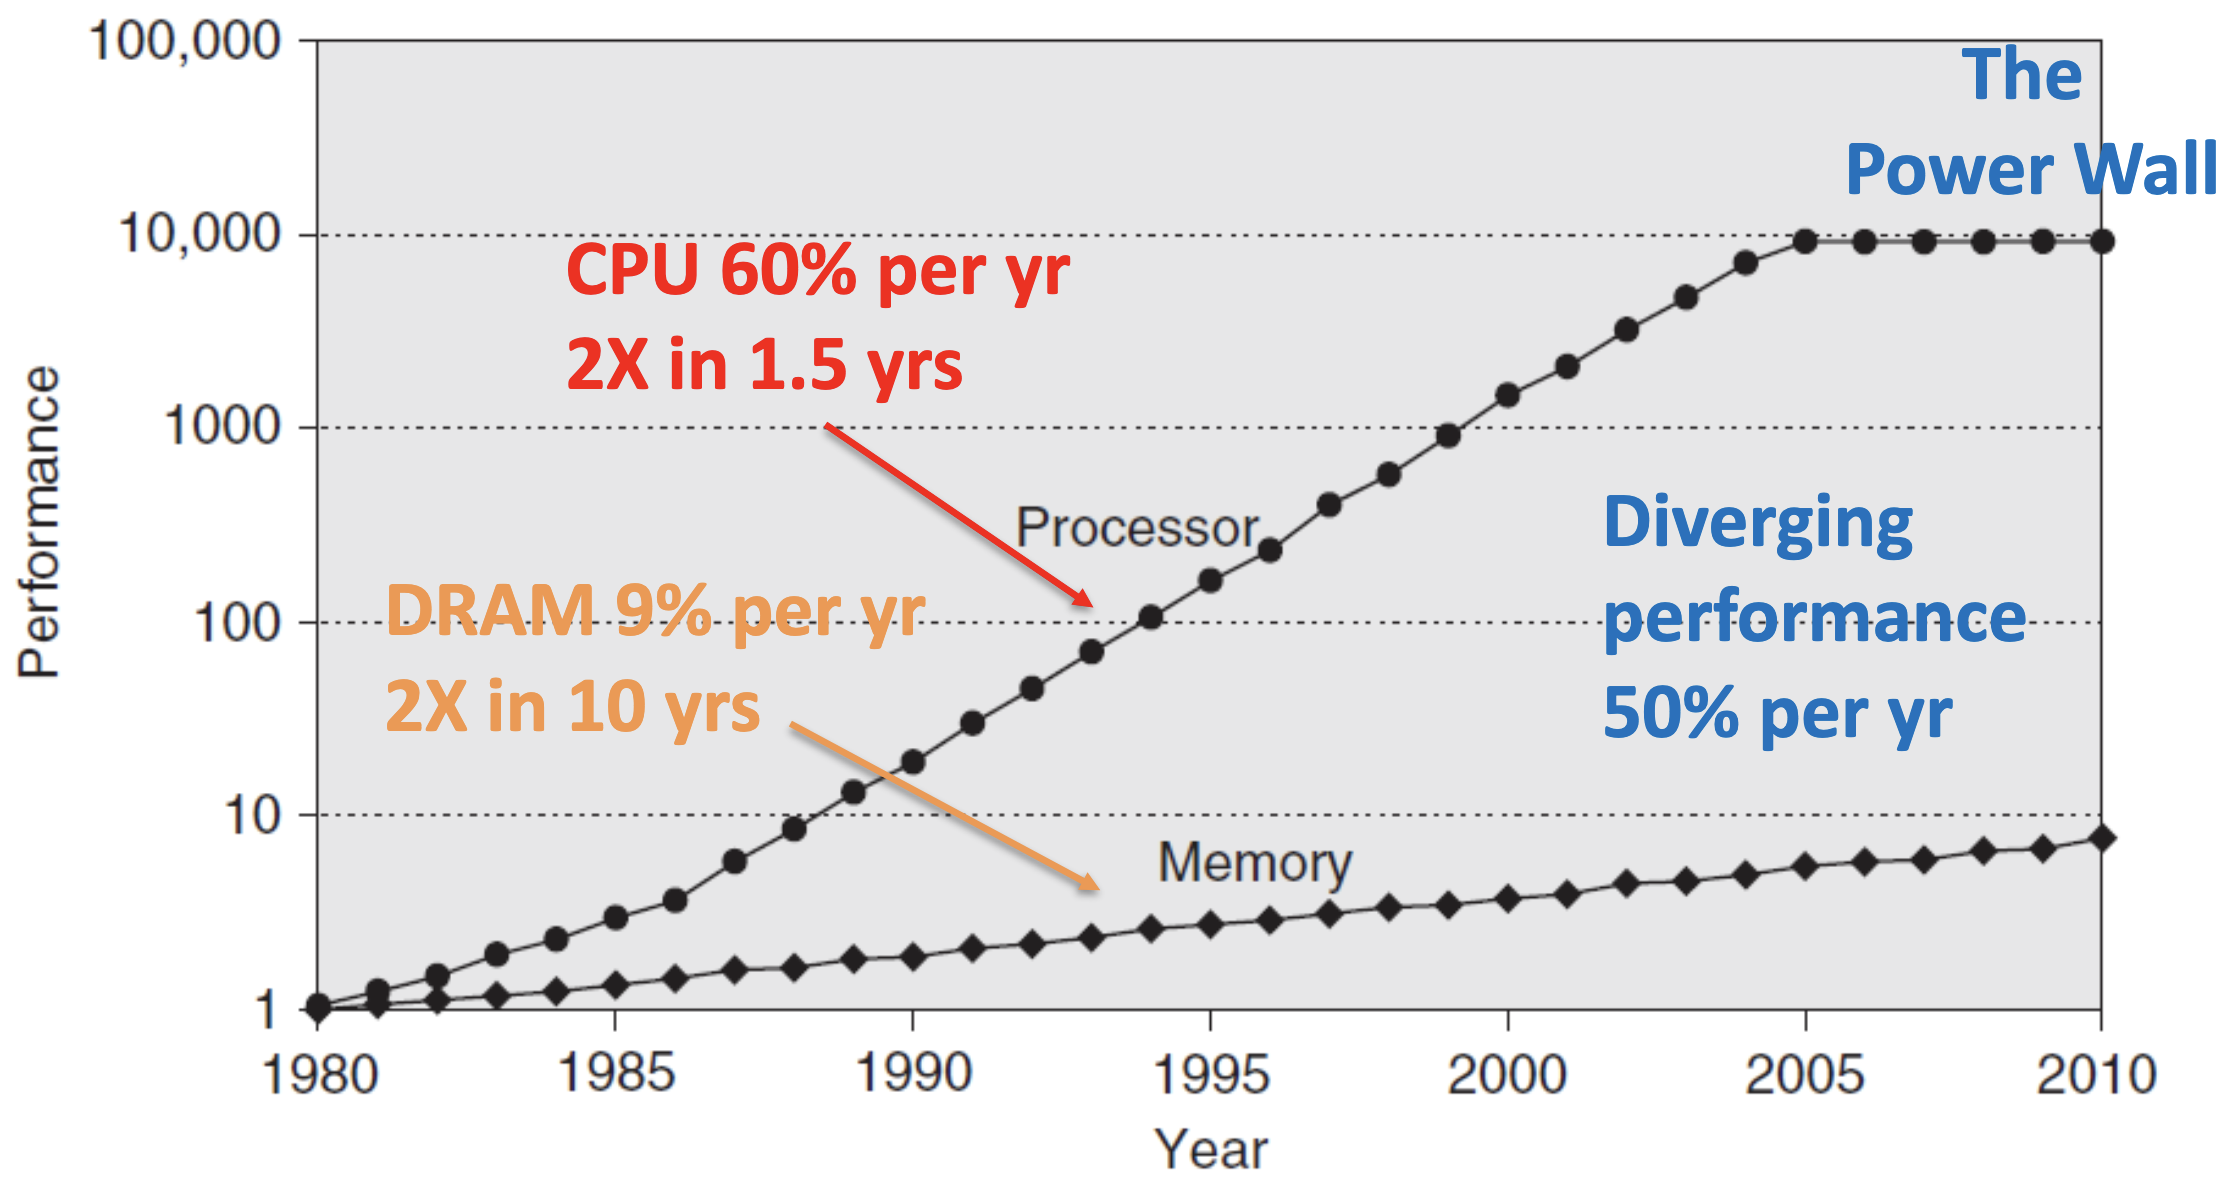
\includegraphics[width=6cm]{images/von-newmann-bottleneck.png}
    \caption{Von-Neumann Bottleneck}
\end{wrapfigure}
L'obiettivo è quindi di fornire l'\textbf{illusione} di avere una memoria grande quanto la memoria più lontana e veloce quanto la memoria più vicina.
Per farlo facciamo risiedere i dati inizialmente nel livello più lontano e più capiente. Per far accedere il processore bisognerà spostare i dati tra i vari livelli di gerarchia.\\
Questo metodo presenta alcune problematiche: serve un meccanismo che, se un dato è già presente un certo livello, determini quello giusto e un meccanismo che permetta di rimpiazzare certi dati per poter fare spazio.\\


\subsection{Terminologia}
Introduciamo ora un po' di terminologia che ci servirà successivamente.

\begin{definition}[Hit e Miss]
Se i dati richiesti dal processore compaiono in qualche blocco nel livello di memoria più vicino, si parla di \textbf{hit}. In caso contrario, si parla di \textbf{miss} e si accede al livello di memoria successivo per recuperare il blocco contenente i dati richiesti.
\end{definition}

\begin{definition}[Hit rate]
    L'hit rate (frequenza di successi) è la frazione di accessi alla memoria rilevati nel livello superiore (ovvero, più vicino alla CPU), utilizzata come misura delle prestazioni della gerarchia.
\end{definition}

\begin{definition}[Miss rate]
    Il miss rate è la frazione di accessi alla memoria non trovati nel livello superiore.
\end{definition}

\begin{definition}[Miss penalty]
    La miss penalty è il tempo necessario per sostituire un blocco nel livello $n$ con il blocco corrispondente dal livello $n-1$.
\end{definition}

\begin{definition}[Miss time]
    Il miss time è il tempo per ottenere l'elemento in caso di tempo di miss. 
    \begin{equation*}
    	\text{miss time} = \text{miss penalty} + \text{hit time}
    \end{equation*}.
\end{definition}

\noindent Il \textbf{miss rate} e l'\textbf{hit rate} si calcolano con le seguenti formule:
\begin{equation}
    MR = \frac{\text{Number of misses}}{\text{Number of total memory access}} = 1 - HR
\end{equation}
\begin{equation}
    MR = \frac{\text{Number of hits}}{\text{Number of total memory access}} = 1 - MR
\end{equation}

\subsubsection{AMAT}
Definiamo l'Average Memory Access Time:
\begin{equation}
    AMAT = t_{M0} + MR_{M0} * (t_{M1} + MR_{M1} * (t_{M2} + MR_{M2} * (t_{M3} + \ldots)))
\end{equation}
$t_{M0}$ = hit time, $MR_{M0}$ = miss rate, $(t_{M1} + MR_{M1} * (t_{M2} + MR_{M2} * (t_{M3} + \ldots))$ = miss penalty.

\begin{observation}
Se l'hit rate è abbastanza alto, la gerarchia della memoria ha un tempo di accesso effettivo vicino a quello del livello più alto (e più veloce) e una dimensione uguale a quella del livello più basso (e più grande).
\end{observation}

\begin{example}
	Consideriamo una memoria con una gerarchia su 3 livelli con i seguenti valori:
	\begin{center}
		\begin{tabular}{|c|c|c|}
			\hline
			\textbf{Livello} & \textbf{Miss rate} & \textbf{Hit time} \\
			\hline
			L1 & 5\% & $t_{L1}$ \\
			L2 & 2\% & $t_{L2}$ \\
			L3 & 100\% & $t_{L3}$ \\
			\hline
		\end{tabular}
	\end{center}
	Quindi il valore AMAT sarà:
	\begin{equation*}
		AMAT= t_{L1} + 0.05 * (t_{L2} + 0.02 * t_{L3}) = t_{L1} + 0.05 * t_{L2} + 0.001 * t_{L3}
	\end{equation*}
\end{example}

\subsection{The locality principle}
Il principio di località di riferimento (o locality principle) si riferisce al fenomeno per il quale un programma tende ad accedere alla stessa locazione di memoria per un determinato periodo.\\
Possiamo osservare che, se il programma fa riferimento ad una locazione di memoria allora:
\begin{itemize}
	\item la stessa locazione di memoria verrà riutilizzerà a breve con alta probabilità
	\item gli elementi "vicini" alla posizione di memoria appena raggiunta saranno presto referenziati con un'alta probabilità
\end{itemize}

Il principio di località è la forza trainante che rende la gerarchia della memoria funzionante. Esso infatti incrementa la probabilità di riutilizzare dei blocchi di dati che erano stati precedente mossi da un livello $n$ ad un livello $n-1$, riducendo il miss rate.\\ Il programmatore dovrà comunque fare attenzione ad implementare questo principio.

\subsubsection{Locality characterization}
Andiamo a distinguere due tipologie di località. 
\begin{itemize}
    \item \textbf{La località temporale} (o riuso di dati): i dati riferiti precedentemente probabilmente verranno riferiti nuovamente in un breve lasso di tempo.
    \begin{example}[Località temporale]
    Consideriamo il seguente codice:
    \begin{lstlisting}
    	for(int i=0; i<10; i++)
    		s1 += i; s2 -= 1;
    \end{lstlisting}
    In questo caso le locazioni di memoria che contengono s1 ed s2 hanno località temporale.
    \end{example}
    Dunque se all'interno della gerarchia della memoria teniamo i dati più recenti, secondo il principio di località ci riaccederò nuovamente dopo poco tempo.
    
    \item \textbf{Località spaziale}: dati vicini a quelli a cui sto facendo riferimento saranno probabilmente utilizzati a breve.
    \begin{example}[Località spaziale]
    	Consideriamo il seguente codice:
    	\begin{lstlisting}
    		for(int i=0; i<10; i++)
    			func(A[i]);
    	\end{lstlisting}
    	In questo caso le locazioni di memoria dell'array hanno località spaziale, visto che sono implementate in modo contiguo.
    \end{example}
    Dunque se all'interno della gerarchia della memoria teniamo i dati vicini a quelli in utilizzo, secondo il principio di località ci saranno grosse probabilità di accedervi con la CPU.
\end{itemize}


\subsection{Traferimiento dati}
I dati si trasferiscono solamente attraverso due memorie adiacenti. Per ottimizzare il caricamento dei dati esso viene fatto come \textbf{blocchi} di dimensione granulare (parole) in modo da poter sfruttare la località spaziale. La dimensione dei blocchi può cambiare attraverso i livelli.\\
Per la cache i blocchi vengono chiamati \textit{cache line} o \textit{cache block} (tipicamente 64-128 bytes, 8-16 parole). Per le RAM invece abbiamo \textit{pagine di segmenti}, mentre per i dischi abbiamo \textit{blocchi di dischi}.\\

\noindent Consideriamo il seguente codice in C e il suo corrispettivo in assembly.
\begin{figure}[!h]
\begin{minipage}[t]{0.45\linewidth}
\centering
\begin{lstlisting}
// Sum and A are global variables
int i;
for(int i=0; sum=0; i<N, i++){
    sum += A[i];
}
\end{lstlisting}
\end{minipage}
\hspace{.35cm}
\begin{minipage}[t]{0.45\linewidth}
\begin{lstlisting}[language={[x86masm]Assembler}]
@ r0=&A, r1=&sum, r2=N, r3=i
loop: cmp r3, r3
      beq end
      ldr r12, [r0, r3, lsl #2]
      ldr r4, [r1]
      add r4, r4, r12
      str r4, [r1]
      add r3, r3, #1
      b loop
end: ...
\end{lstlisting}
\end{minipage}
\end{figure}

In questo frammento di codice il loop viene eseguito N volte, e quindi ogni struttura viene richiesta N volte in maniera sequenziale. In questo caso sia la localizzazione temporale che spaziale viene utilizzata.\\
'Sum' è ripetutamente letta e scritta, quindi utilizza la località temporale, 'A' è salvata come un insieme contiguo di celle di memoria, quindi utilizza la località spaziale.

\subsection{Cache}
La cache memory è la memoria più vicina al processore, solitamente sono le SRAM, ma alcune volte sono implementate anche come DRAM. Ad oggi tutte le architetture hanno alcuni livelli di cache integrati nel chip, essa può essere più o meno grande e può avere più di un livello.

\subsubsection{Gestione del movimento dei dati}
Fra il primo livello di cache e i registri il trasferimento è gestito dal compilatore. Il trasferimento fra caches e RAM viene invece gestito dalla microarchitettura. Infine la gestione dei trasferimenti fra RAM e storage viene fatta dal sistema operativo.

\begin{figure}[h!]
    \centering
    \begin{subfigure}{.45\textwidth}
        \centering
        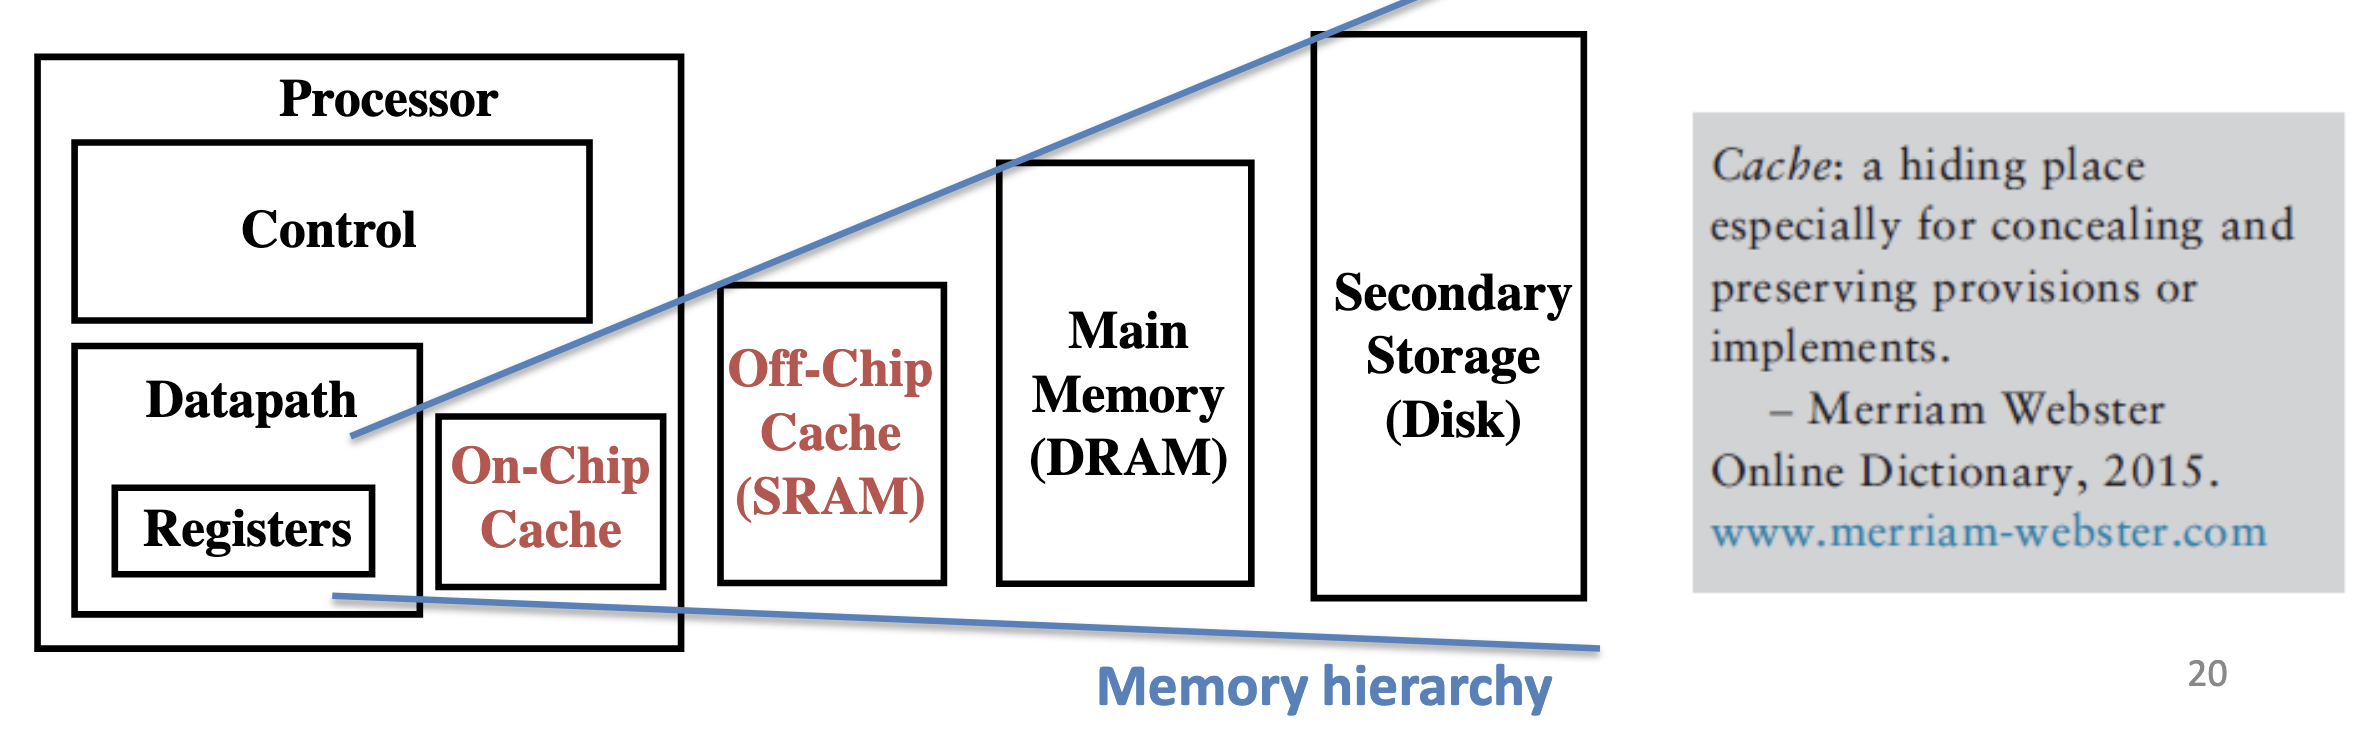
\includegraphics[width=6.5cm]{images/cache-memories.png}
        \caption{}
    \end{subfigure}
    \begin{subfigure}{.45\textwidth}
        \centering
        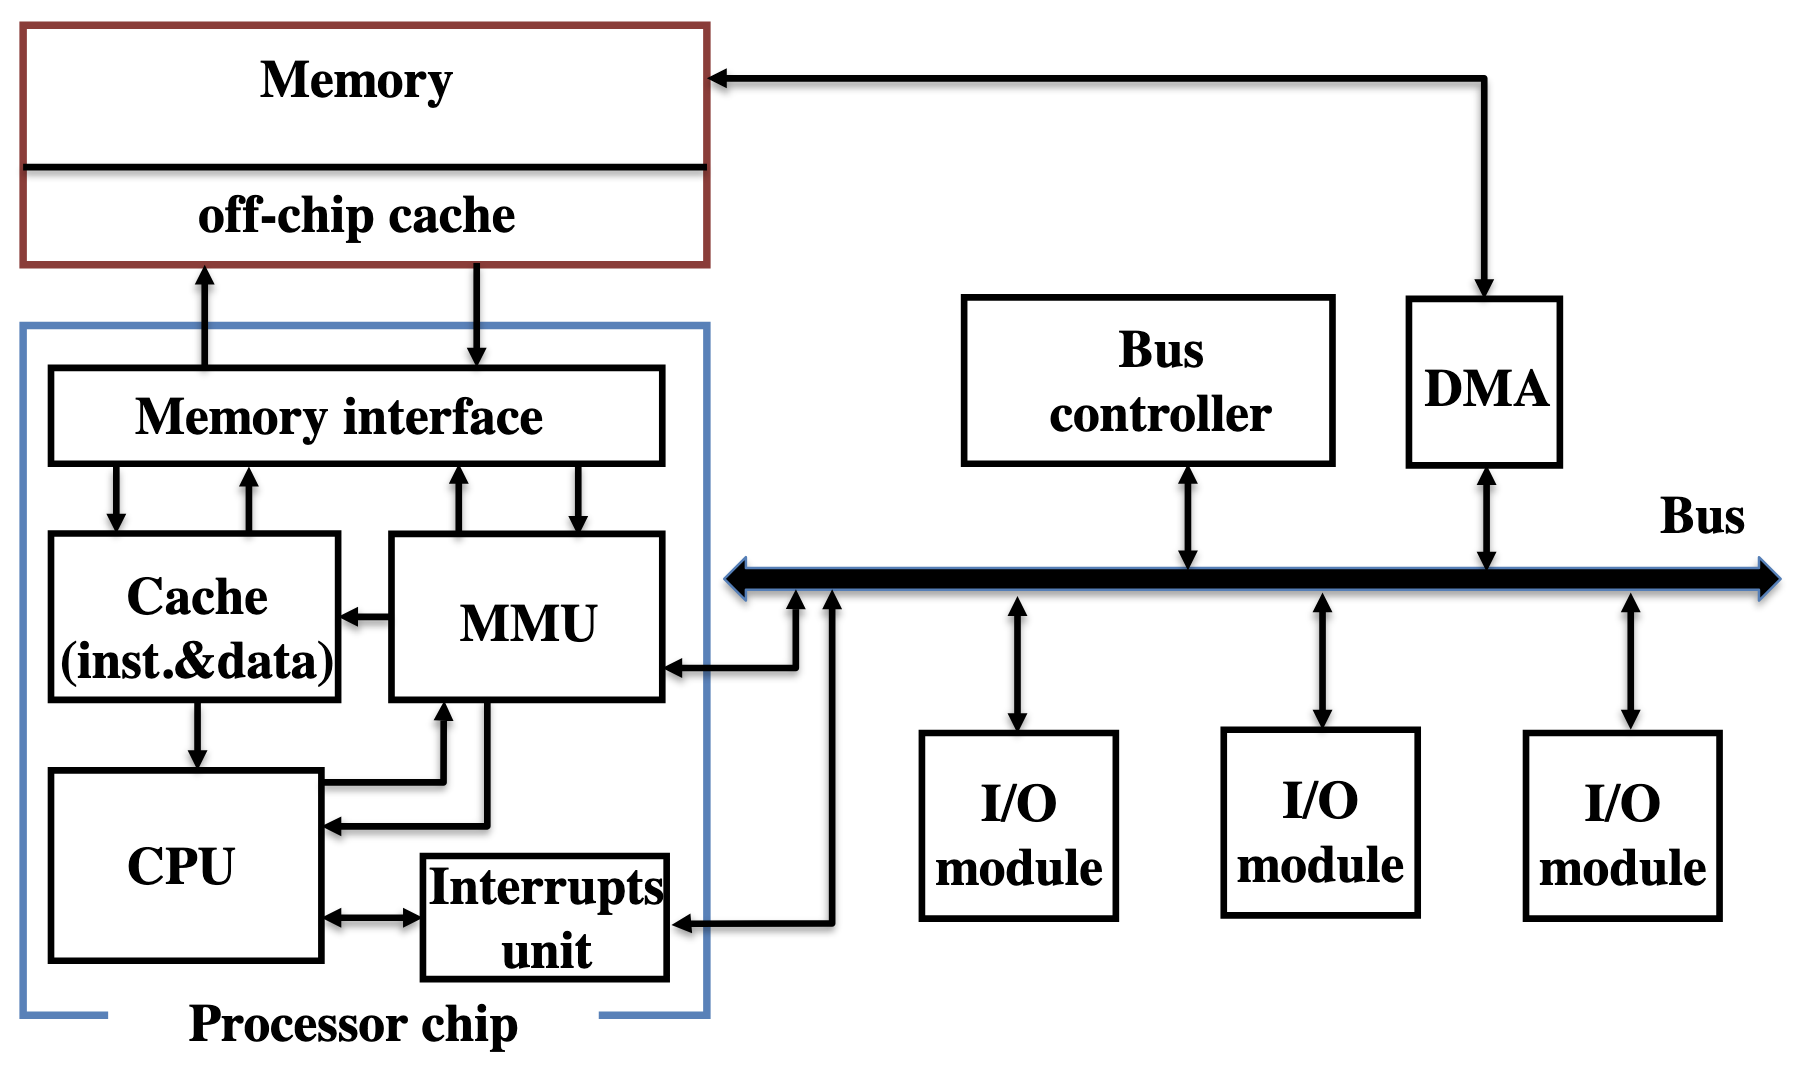
\includegraphics[width=6.5cm]{images/cache-based-architecture.png}
        \caption{}
    \end{subfigure}
\end{figure}
    

\subsubsection{Utilizzo}
L'organizzazione della cache avviene non a blocchi ma a linee. Ogni linea contiene blocchi di memoria (8-16 memory words). La prima volta che il processore richiede la memory word avviene una \textbf{cache miss}. A quel punto il blocco contenente la parola viene trasferito dentro la cache.\\
La richiesta successiva può essere di due tipologie:
\begin{itemize}
    \item \textbf{Cache hit}: se il dato è presente nel blocco.
    \item \textbf{Cache miss}: se il dato non è presente dentro il blocco. In questo caso il blocco che contiene il dato viene trasferito dentro la cache line.
\end{itemize}

Vediamo ora l'effetto della cache sull'AMAT. Innanzitutto l'utilizzo di grandi cache nella gerarchia delle memorie aiuta a ridurre il bottleneck di von Neumann. 
\begin{example}
Vediamo un esempio quantitativo stabilendo dei valori:\\
$t_M = 50ns$ (main memory service time), $t_{L1} = 1ns$ (L1 hit time, cache hit service time). \\\\
Abbiamo un Miss rate ($MR_{L1}$) del $5\%$.\\
Senza cache $AMAT = 50ns$ mentre con L1 cache $AMAT = t_{L1} + MR_{L1} * t_M = 1 + 0.05 * 50 = 3.5ns$
\end{example}

\subsubsection{Performance}
\begin{equation}
	CPU_{time} = \text{ClockCycles} \cdot \text{ClockCycleTime} = IC \cdot CPi \cdot \text{ClockCyleTime}
\end{equation}
dove
\begin{itemize}
    \item \textbf{IC} (Instruction Count) è il numero di istruzioni che vengono effettivamente eseguite
    \item \textbf{CPI} (ClockCycles Per Instruction) è definito come \(\frac{clockcycles}{IC}\)
\end{itemize}
Possiamo inoltre dividere il $CPU_{time}$ tra \textbf{$CPI_{Perfect}$}, ovvero il tempo che la CPU impiega per eseguire un'istruzione senza \emph{misses}, e \textbf{$CPI_{Stall}$}, ovvero il tempo che la CPU impiega per aspettare la memoria.
\begin{equation}
	CPU_{time} = (CPI_{Perfect} + CPI_{Stall}) \cdot \text{ClockCycleTime}
\end{equation}
Le due parti le possiamo calcolare come segue:
\begin{equation}
	\begin{split}
		CPI = \bigg(\frac{IC_{CPU}}{IC}\bigg) \cdot CPI_{CPU} + \bigg(\frac{IC_{MEM}}{IC}\bigg) \cdot CPI_{MEM} \\
		CPI_{MEM} = CPI_{MEM-HIT} + \text{Miss Rate} \cdot CPI_{MEM-MISS} \\
		\mathbf{CPI_{Perfect}} = \frac{IC_{CPU}}{IC} \cdot CPI_{CPU} + \frac{IC_{MEM}}{IC} \cdot CPI_{MEM-HIT} \\
		\mathbf{CPI_{Stall}} = \frac{IC_{MEM}}{IC} \cdot \text{Miss Rate} \cdot \text{Miss Penalty}
	\end{split}
\end{equation}

\begin{observation}
	IL $CPI_{Stall}$ è definito come la somma dei cicli di stallo in lettura e scrittura. Per semplicità abbiamo assunto che i miss rate e le miss penalties fossero identiche per lettura e scrittura e che gli stalli per scrivere nei buffer fossero trascurabili.
\end{observation}

\begin{example}
    Assumiamo che abbiamo un miss rate del \(2\%\) per la cache delle istruzioni mentre un \(4\%\) per la cache dei dati, ed una miss penalty di $100$ cicli per ogni mancanza. Una frequenza del \(36\%\) per le \emph{ldr}, e le \emph{str}. Se la CPI è $2$ senza memory stalls, dobbiamo determinare quanto va più veloce un processore con una cache perfetta rispetto ad una cache reale (che ha le caratteristiche elencate sopra).\\

    \[CPI_{Stall-Instr} = 1 \cdot 0.02 \cdot 100 = 2 cycles\]
    \[CPI_{Stall-Data} = 0.36 \cdot 0.4 \cdot 100 = 1.44 cycles\]
    \[CPi_{stall} = 2 + 1.44 = 3.44\]
    spendiamo in media $3.44$, e quindi in totale il nostro processore $CPI = 2 + 3.44 = 5.44$.

    \[\frac{CPU_{\text{time with stalls}}}{CPU_{time Perfect}} = \frac{(CPI_{Perfect} + CPI_{Stall}) \cdot Clockcycletime}{CPI_{perfect} \cdot ClockCycleTime} =  \frac{5.44}{2}\]
\end{example}

Come abbiamo visto nell'esempio è quindi importante tenere bassi:
\begin{itemize}
	\item \textbf{Hit-time}, che deriva dalla tecnologia utilizzata per la cache
    \item \textbf{Miss penalty}, che deriva dall'architettura utilizzata
    \item \textbf{Miss rate}, che può essere abbassato anche tramite tecniche di programmazione
\end{itemize}

\subsection{Design}
Una delle prime domande che dobbiamo porci è come i dati sono organizzati.\\
Partiamo da una cache di una capacità C, organizzata come S sets in cui ciascuno contiene B block (o linee), dove b è il numero di parole per blocco. Tutto questo in un sistema a $32$bit (quindi al massimo possiamo indirizzare $2^{30}$ parole).\\
Da qui possiamo distinguere vari metodi di organizzazione:
\begin{enumerate}
    \item \textbf{Direct mapped}: in questo caso $\#S=\#B$
    \item \textbf{N-way set-associative}, in cui N definisce il numero di blocchi contenuti in un set quindi $S=B/N$
    \item \textbf{Fully associative}, in cui nell'insieme c'è uno unico blocco contenente tutta la cache, quindi $S=1$
\end{enumerate}

\subsubsection{Direct mapped}
Supponiamo di avere $b=1$\footnote{Nessuna cache avrà mai b=1, è solo come esempio} e una cache di 8 parole, quindi $S=B=8$, $C=B\cdot b=8$. Per indirizzare le 8 parole ci serviranno $\log_2 8 = 3$bits.\\

\begin{wrapfigure}{r}{6.5cm}
	\centering
	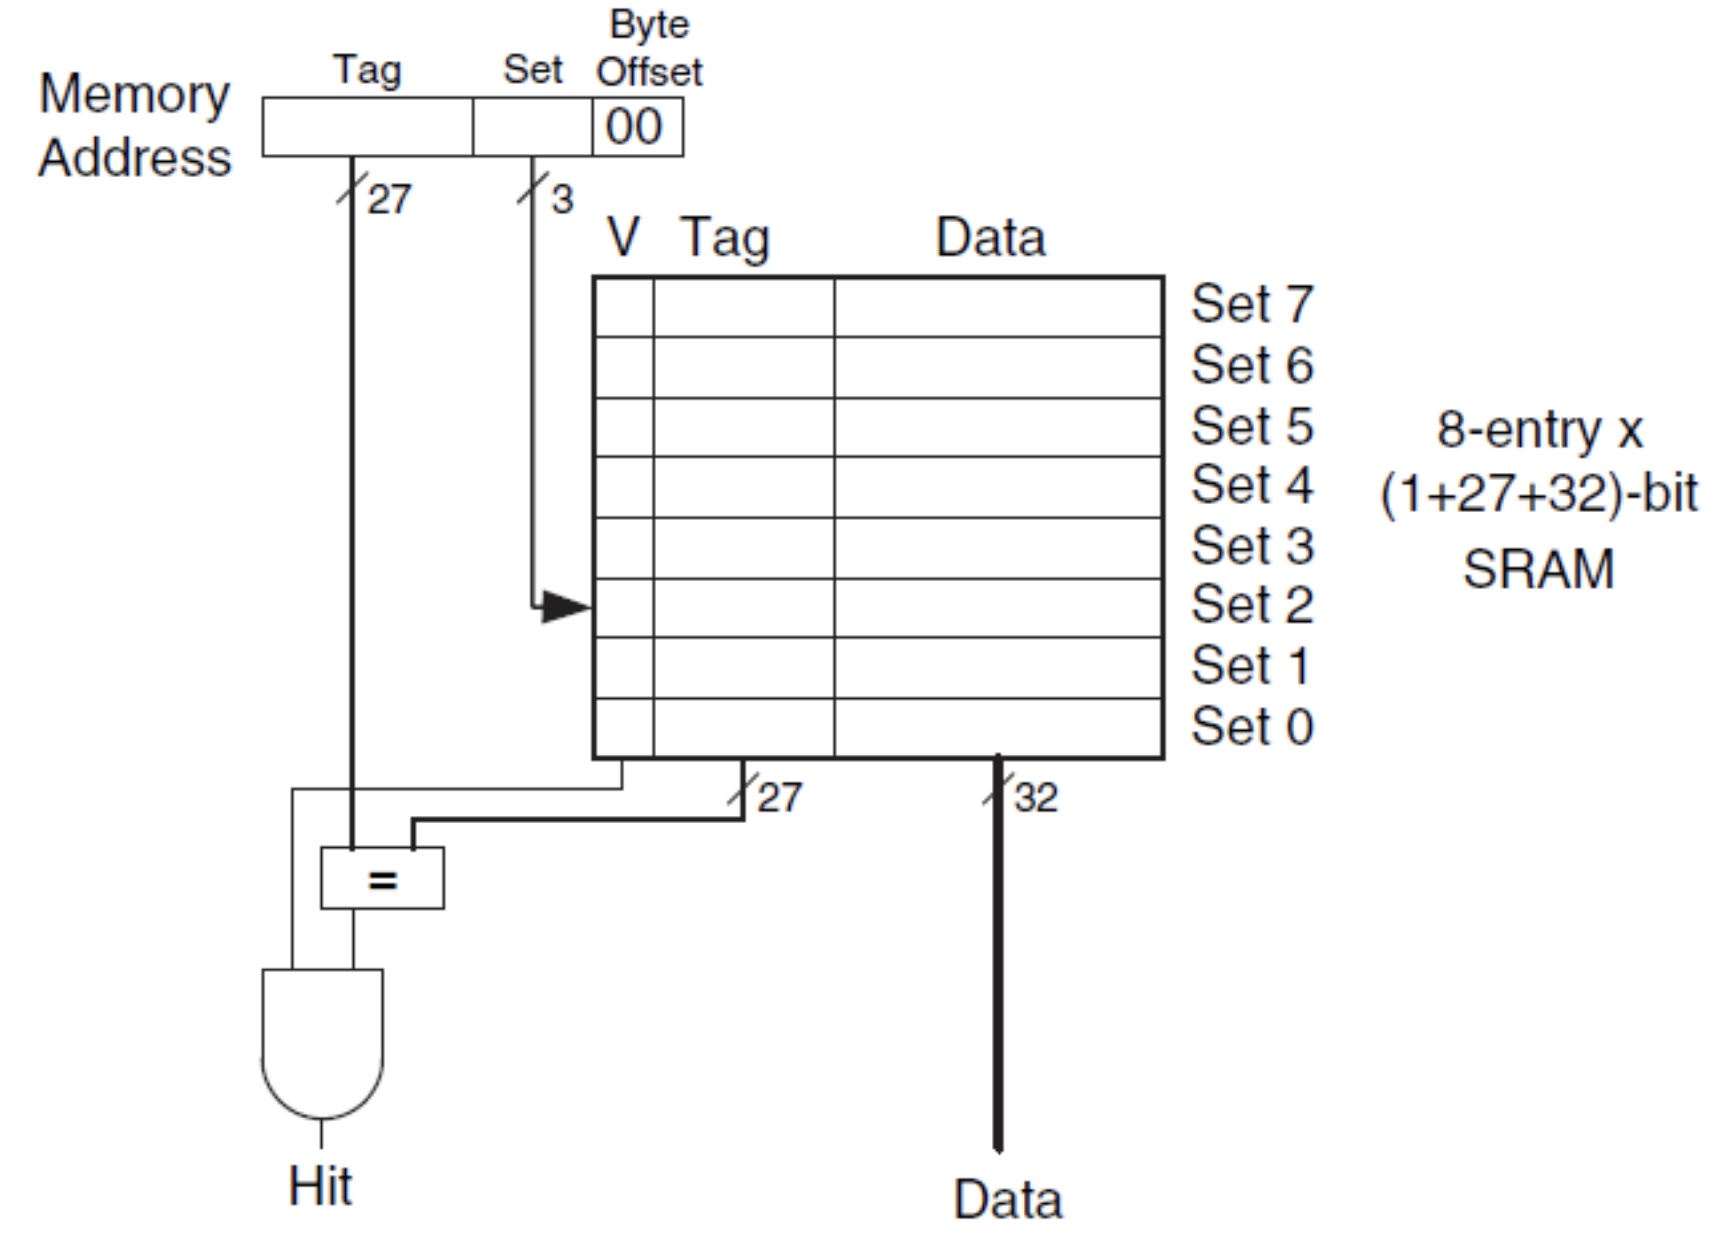
\includegraphics[width=4.5cm]{images/direct-mapped.png}
	\caption{Direct mapped, $b=1$}
\end{wrapfigure}

In questo tipo di design, tutti gli indirizzi con il quintultimo, quartultimo e terzultimo bit in comune saranno associati ad un set nella cache predefinito. \\
In aggiunta nella cache sarà pesente anche un \textbf{tag} che permette di identificare univocamente il dato e un valore di \textbf{controllo} che mi garantisca che quel dato sia effettivamente valido per quella posizione di cache (ad esempio appena acceso il computer potrebbe esserci un valore random non corretto).\\

\noindent Vediamo un caso realistico dove \(b > 1\). Prendiamo $C = 8$ e $b = 4$,con $B = C/b = 2$ e $S = 2$. Dobbiamo quindi andare af "affettare l'indirizzo" aggiungendo un \textbf{block-offset} che mi permetta di selezionare la parola corretta tra le $\log_2 4$ opzioni
\begin{center}
	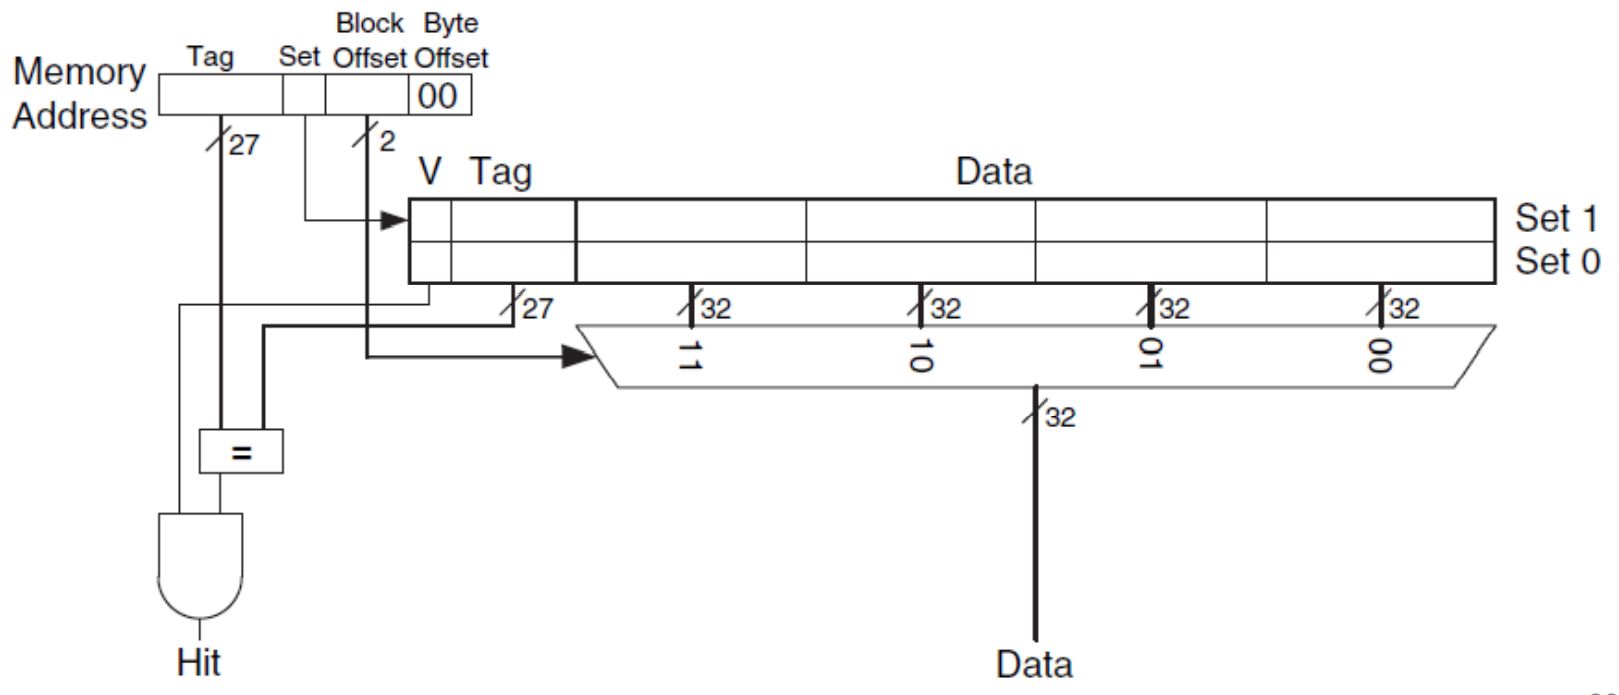
\includegraphics[scale=0.15]{images/direct_mapped_2.png}
\end{center}

\noindent Per implementare anche la scrittura in un indirizzo, aggiorniamo lo schema come segue:
\begin{center}
	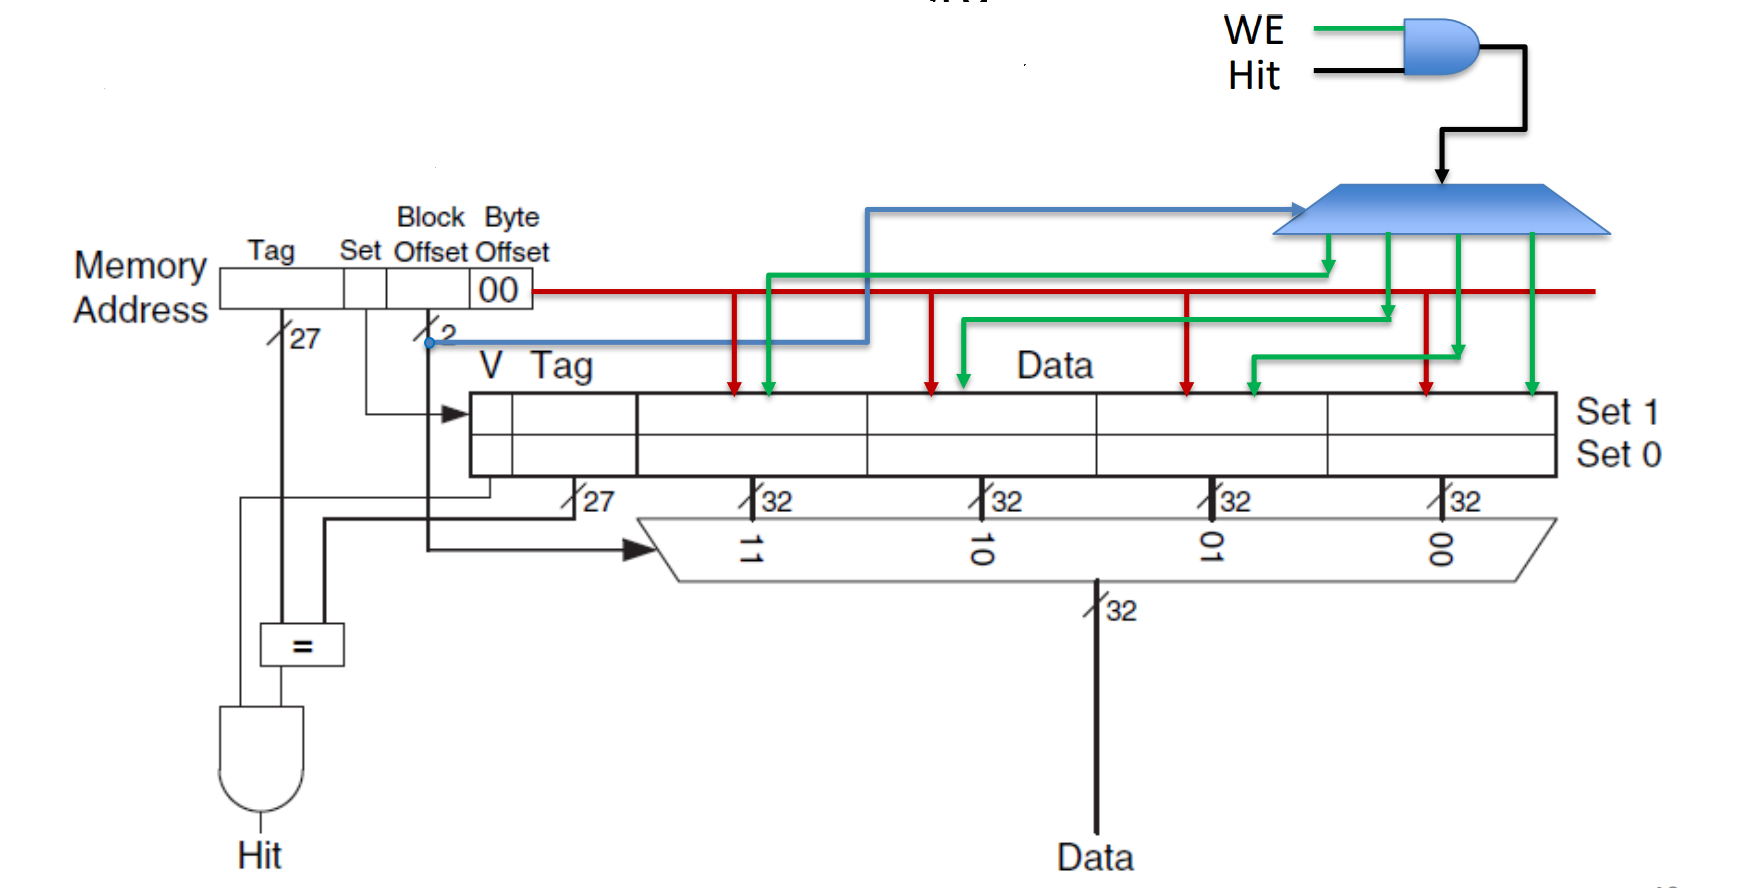
\includegraphics[scale=0.15]{images/direct_mapped_3.png}
\end{center}

\begin{example}
	\label{example:direct_access_1}
    Supponiamo di avere indirizzi a $32$bit, una cache ad accesso diretto con $S = B = 128$ ed ognuna contiene $b = 8$. Dobbiamo trovare la struttura con cui organizzare gli indirizzi.\\
    Ci servono $2$bit per l'offset del dato, $log_2 8=3$bit per l'offset delle parole nel blocco, \(\log_2 129 = 7\)bit per identificare il \emph{set} e 20bit per il tag del dato.
    \begin{center}
    	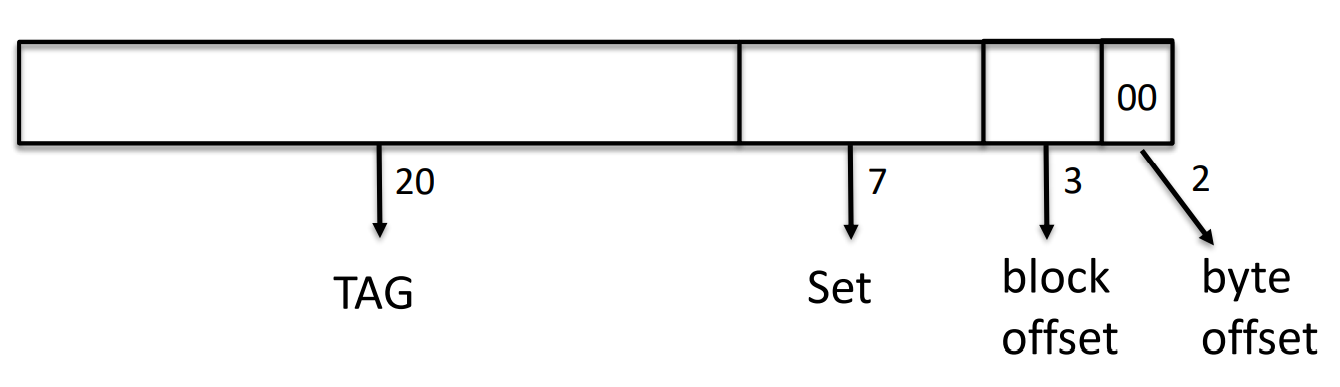
\includegraphics[scale=0.1]{images/direct_mapped_example_1.png}
    \end{center}
\end{example}

\begin{example}
   Consideriamo la stessa struttura dell'esempio \ref{example:direct_access_1}. Dobbiamo calcolare la linea di cache e l'offset all'interno della linea
    di cache che conterrà l'indirizzo 0xFFAC.\\
    \begin{equation*}
    	\text{0xFFAC} = 0\ldots01111 \color{red}1110 101\color{green}0 11\color{blue}00\color{black} 
    \end{equation*}
    L'indirizzo si dividerà quindi in:
    \begin{itemize}
    	\item Tag
    	\item \color{red}Set\color{black}
    	\item \color{green}Block offset\color{black}
    	\item \color{blue}Byte offset \color{black}
    \end{itemize}
    Quindi la linea di cache ha indice 117, ovvero 118esima. L'offset nel blocco è 3 quindi la quarta parola di memoria.
\end{example}

\begin{example}
    Consideriamo il seguente codice in C:
    \begin{lstlisting}[language=C]
    	for(i=0; i<16, i++)
    		C[i] = A[i] + B[i];
    \end{lstlisting}
    eseguito in un processore a 2Ghz con un mapping diretto L1 ai dati dalla cache con $C = 128$, $b=8$, \(t_M = 100\) cicli e \(t_{L1} = 4\) cicli.\\
    'A' inizia all'indirizzo 0x00000000, 'B' inizia all'indirizzo 0x00000040 e 'C' inizia all'indirizzo 0x00000080. Calcolare il numero di cache misses e l'AMAT considerando solo le \emph{ldr}.\\\\
    Il primo passo è verificare se A e B finiscono nello stesso set: A verrà caricato nel set 0 e nel set 1 mentre B nel set 2 e nel set 3, quindi non vanno in conflitto.
    Se supponiamo la cache sia vuota: avremo 4 cache misses, due per ogni word di A e B, e 32 cache hits (12 per A e 12 per B).\\
    Il calcolo dell'AMAT sarà
    \begin{equation*}
    	\begin{split}
    		&MissRate = \frac{4}{32}\\
    		&CloclCycleTime=\frac{1}{2GHz}=0.5ns\\
    		&AMAT=\bigg(4+\frac{4}{32} \cdot 100\bigg) \cdot ClockCycleTime = 8.25ns
    	\end{split}
    \end{equation*}
    In generale, se non c'è \textbf{località temporale}, il numero di cache misses è $\frac{N}{b}$, dove $N$ è il numero di istruzioni (in questo caso $N=2\cdot16$).
\end{example}

\noindent Per riassumere possiamo dire che i pro sono:
\begin{itemize}
    \item La realizzazione è semplice
    \item E' molto veloce in caso di hits
\end{itemize}
mentre i contro:
\begin{itemize}
    \item La funzione di mapping a posizione fisse può generare potenzialmente molti conflitti.
    \item La troppa rigidità potrebbe avere un grosso impatto sul numero dei conflitti nella cache (\textbf{trashing}) in quanto essi dipendono dal posizionamento della memoria e dall'utilizzo delle strutture dati.
\end{itemize}

\begin{definition}[Working set]
	Data una gerarchia di memoria M1-M2, il working set di un programma è l'insieme dei dati che, se simultaneamente presenti in M1, massimizza la probabilità di hits in M1.
\end{definition}

\begin{example}[Working set]
	Prendiamo per esempio il seguente codice:
	\begin{lstlisting}[language=C]
		// A and B are two arrays of size N
		// (the cache block b << N)
		for(i=0; i<N; ++i)
			for(j=0; j<N; ++j)
				A[i] = F(A[i], B[j])
	\end{lstlisting}
	in cui l'array A ha località spaziale e temporale e B quella spaziale (sul lungo termine anche temporale).\\
	Il nostro WS sarà l'elemento corrente di A e l'intero array B. Quindi, se la cache contenesse il WS avremmo solamente $O(\frac{N}{b})$ fallimenti.
\end{example}

\begin{figure}[h!]
    \centering
    \begin{subfigure}{.45\textwidth}
        \centering
        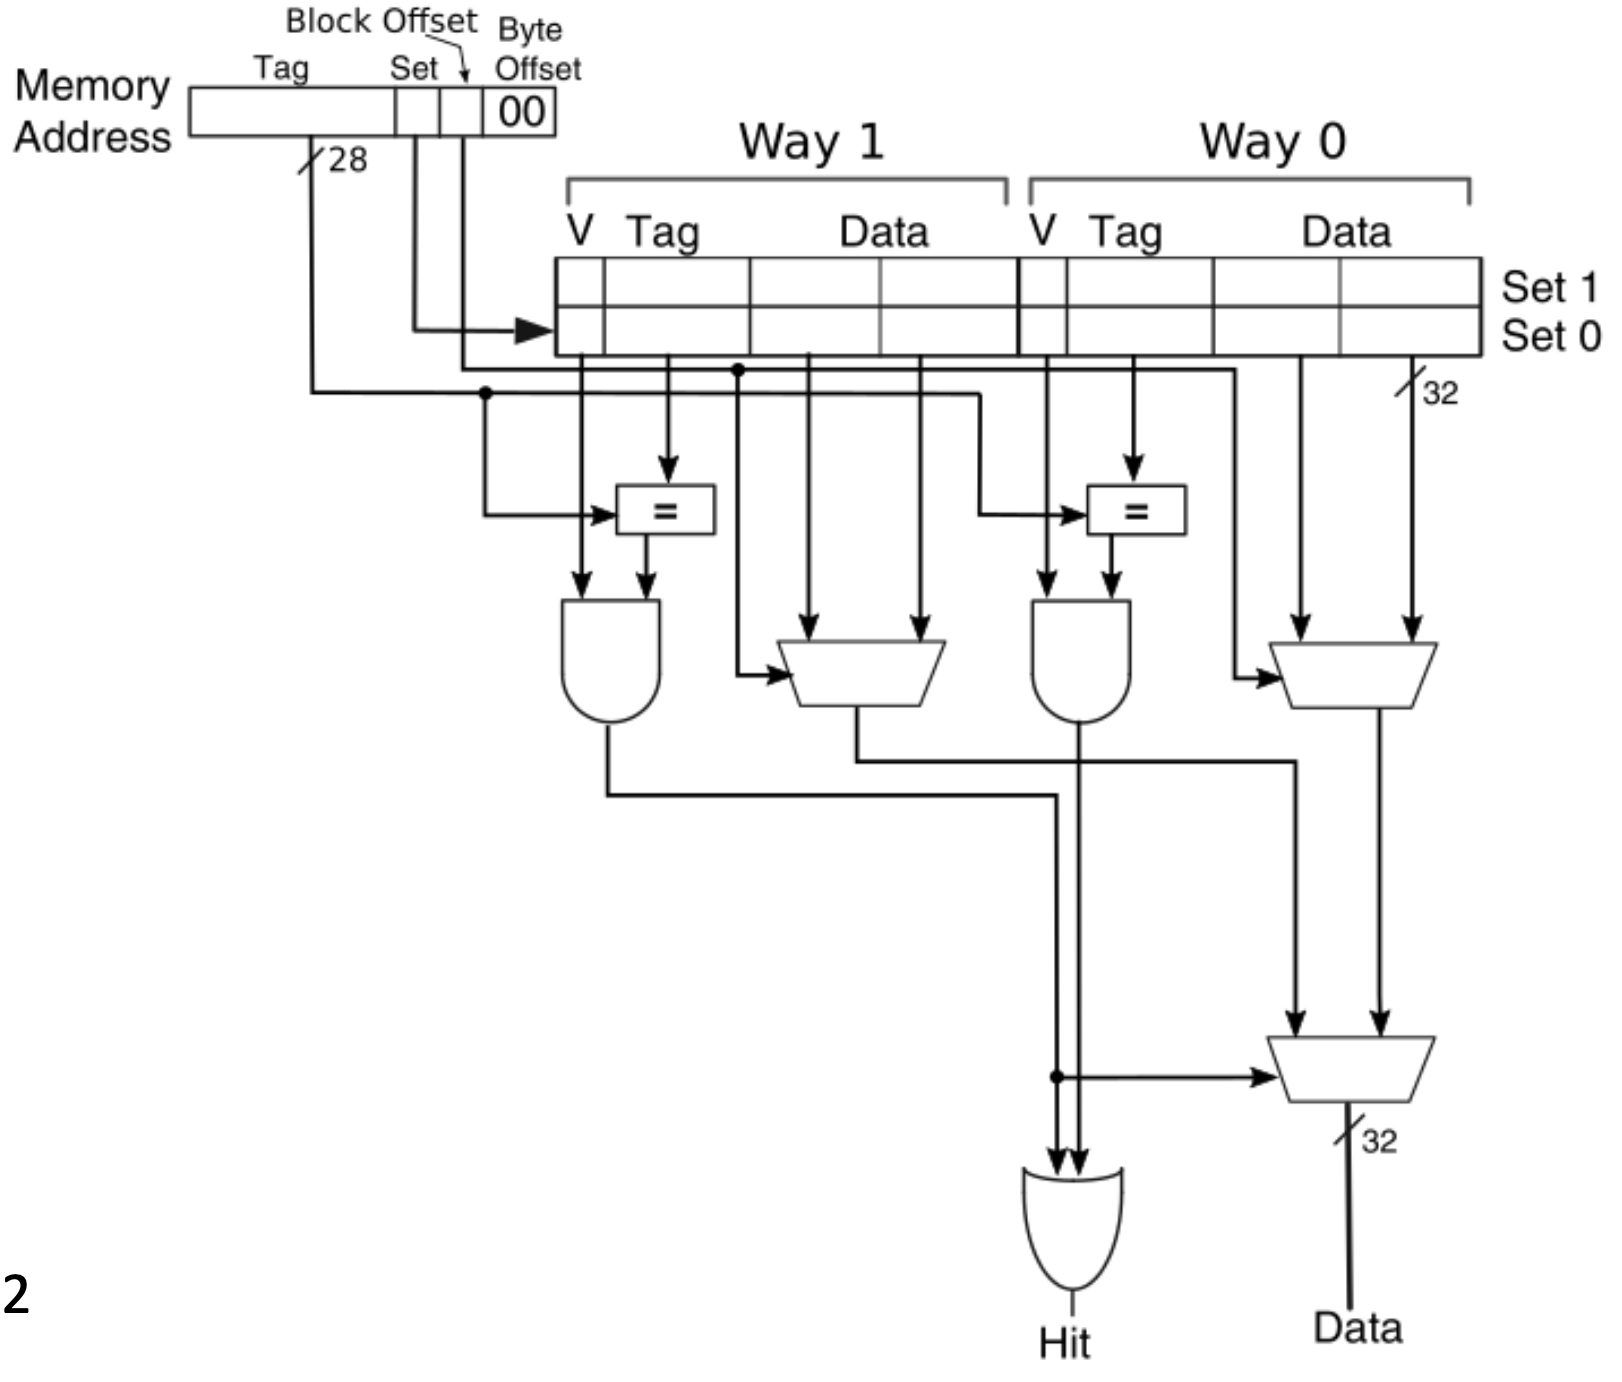
\includegraphics[width=4.7cm]{images/fully-associative.png}
        \caption{Fully associative}
    \end{subfigure}
    \begin{subfigure}{.45\textwidth}
        \centering
        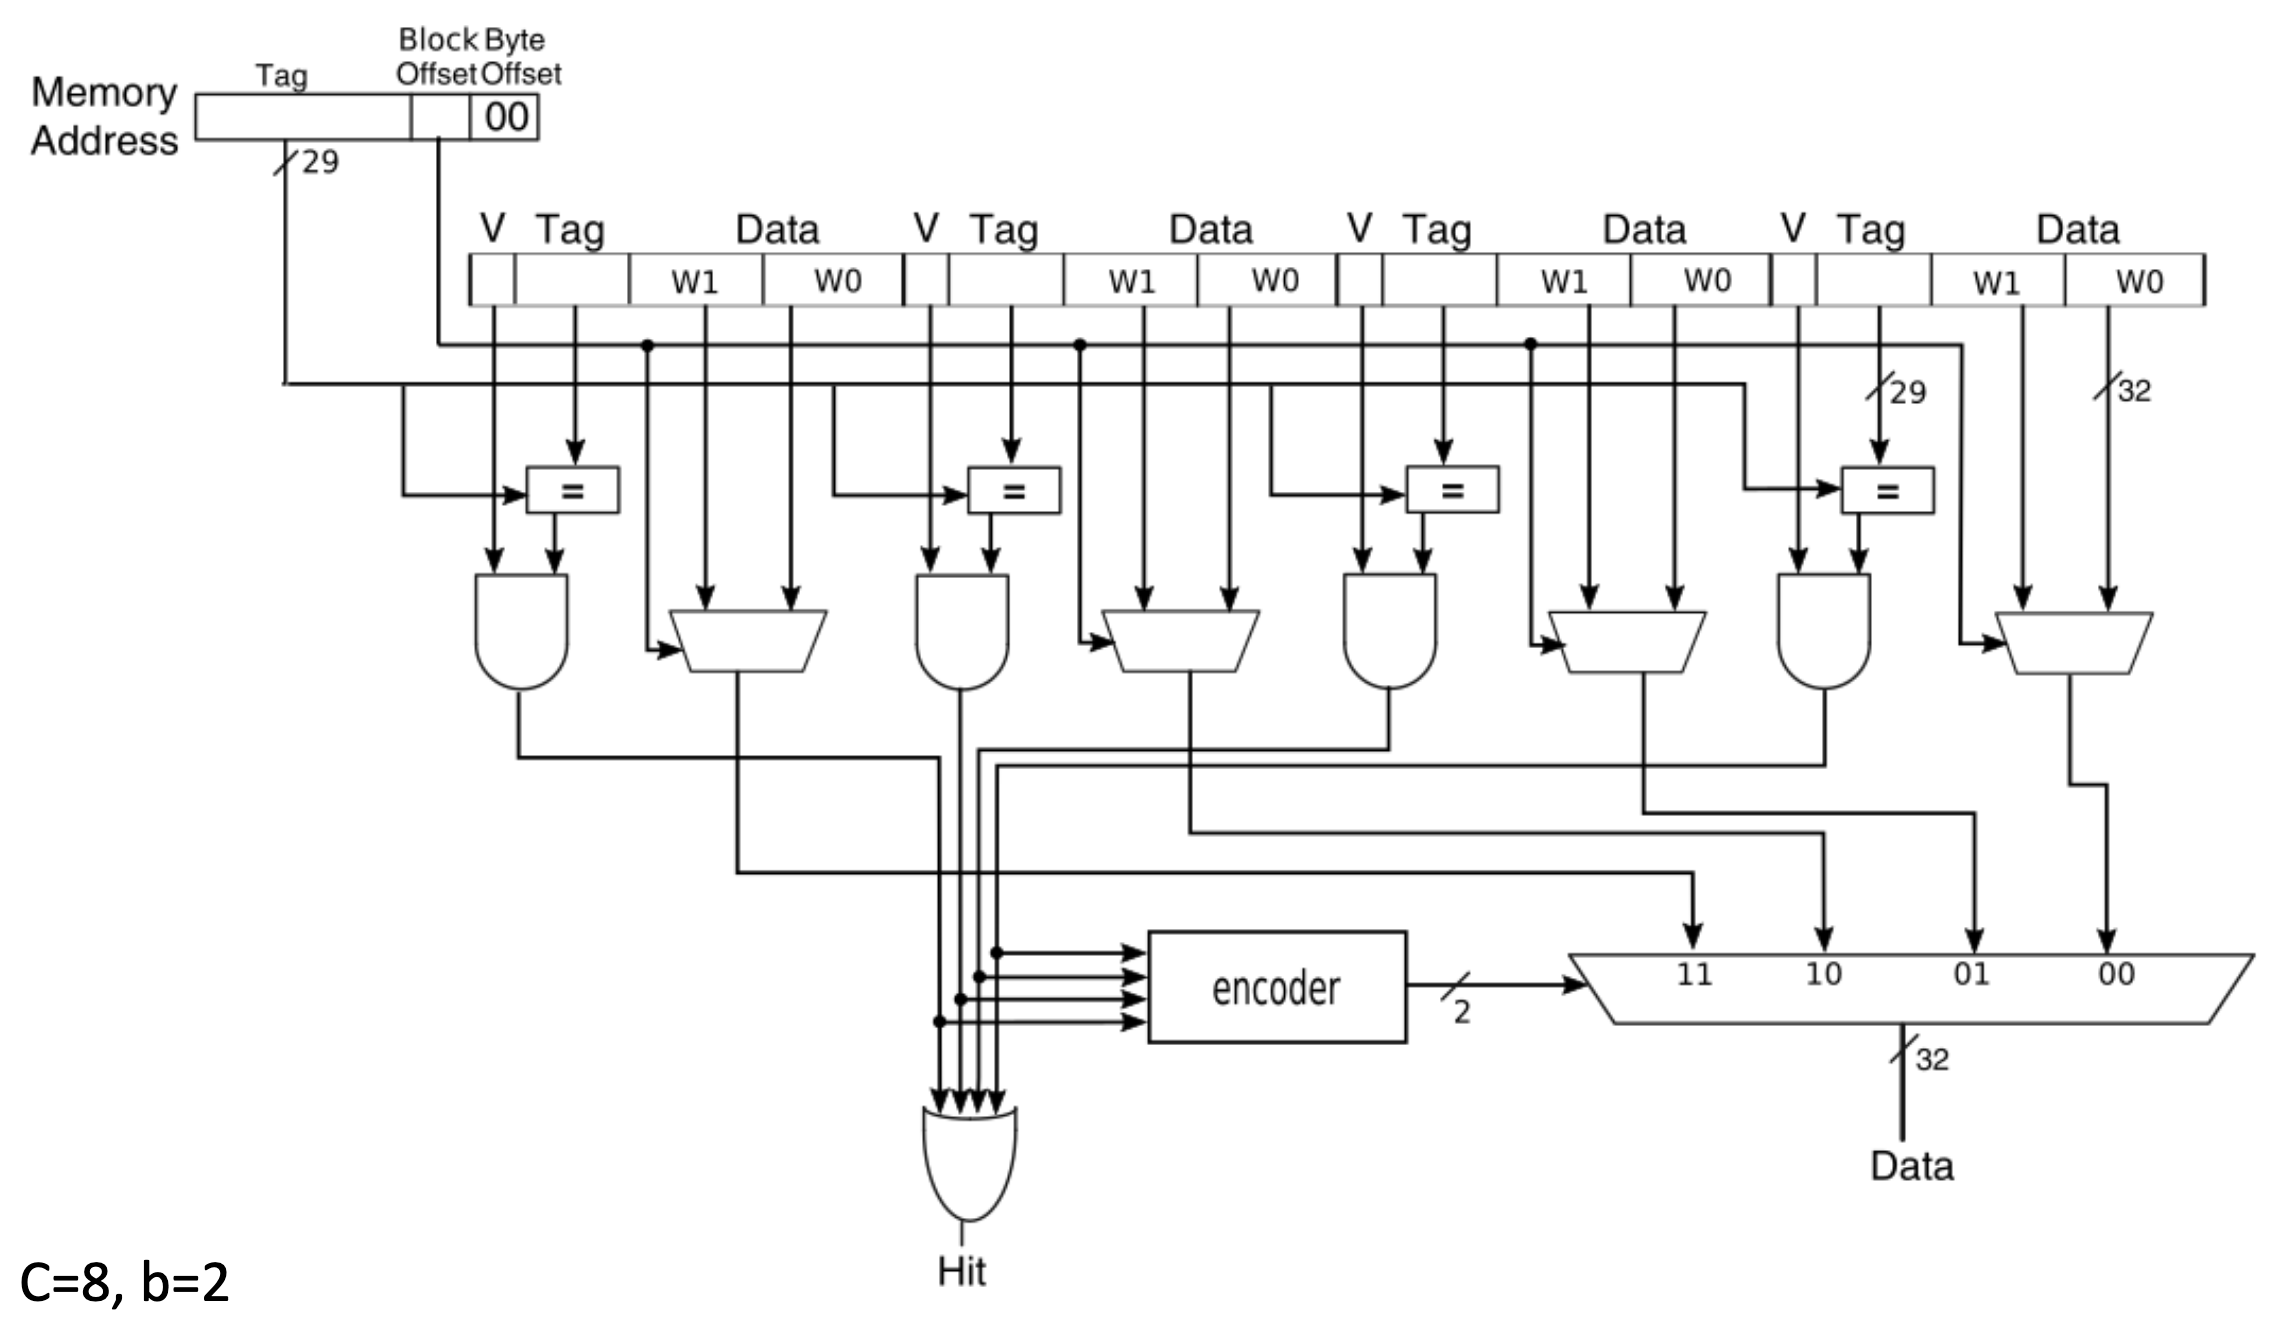
\includegraphics[width=4.7cm]{images/n-way-associative.png}
        \caption{N-way associative}
    \end{subfigure}
\end{figure}


\subsection{Cache miss}
Le tipologie di cache miss sono le seguenti:
\begin{itemize}
    \item \textbf{Compulsory miss} questo tipologia di cache misses viene causato dal primo acceso al blocco che non è mai stato in cache.
    \item \textbf{Capacity miss} causato dalla cache che non coneinte tutti i bocchi necessari.
    \item \textbf{Conflict miss} solo per la mappatura diretta per i set associativi
\end{itemize}
A questo punto, visti i vari strumenti della cache e le tipologie di miss possnaimo andare  avedere come ridurre i cache miss tramite l'utilizzo di alcune tecniche:
\begin{itemize}
    \item \textbf{Aumentare la dimensione dei blocchi}. Andando così ad unmentare la località spaziale ma umentando anche la miss penalty.
    \item \textbf{Aumenteare l'associativià}. Meno conflitti ma un maggiore tempo di hit.
    \item \textbf{Aumentare dim. dei case}. Porta a meno capacity miss e conflitti ma aumenta l'hit time.
    \item \textbf{Usare algoritmi di cache-oblivius}.
\end{itemize}
In caso comunque avvengano dobbiamo andarli a gestire. Un errore nella cache blocca l'intero processore, congelando 
il contenuto di tutti i registri durante l'attesa della memoria: in effetti, un processore più avanzato consente l'esecuzione fuori ordine di altre istruzioni durante l'attesa della memoria.
Gli steps che vengono eseguiti per la gestione di un cache miss (\textbf{fautl management}):
\begin{enumerate}
    \item Indica al livello di memoria successivo di leggere il valore mancante.
    \item Attendi che la memoria risponda (questo può richiedere più cicli).
    \item Aggiorna la riga della cache corrispondente con i dati ricevuti.
    \item Riavvia l'esecuzione dell'istruzione (ora è un hit della cache).
\end{enumerate}


\subsection{Gestione delle scritture}
Dobbiamo definire quelle che sono le \textbf{write hits}, se l'istruzione di stroe scribe il dato soltanto dentro la cache, dopo la cache
è la memoria potrebbeero avere differenti valori (quindi abbiamo un inconsistenza).\\
Abbiamo poi \textbf{write miss}. 
\begin{itemize}
    \item Chiediamoci se possiamo recuperare il blocco dalla memoria alla cache e poi andiamo a sovrascivere la parola mancante?
    La risposta è si e questa policy si chiama \textbf{write-allocate}.
    Il blocco viene caricato nella cache seguito da un hit di scrittura (utilizzato principalmente nella politica Write-Back).
    \item Poi chiediamoci anche se dovremmo scrivere la parola direttamente al livello di memoria successivo? 
    Questa politica è chiamata \textbf{no-write-allocate}, il blocco non viene caricato nella cache (utilizzato principalmente nella politica Write-Through)
\end{itemize}

\subsubsection{Write-Through}
Gli hit di scrittura aggiornano sempre sia la cache che il successivo livello di memoria.
\begin{itemize}
    \item \textbf{Pro}: Soluzione semplice, facile da implementare. I dati sono sempre coerenti tra i due livelli di memoria.
    \item \textbf{Contro}: La velocità di scrittura dipende dalla velocità di scrittura del livello di memoria inferiore. Maggiore traffico di memoria, per ogni singola scrittura potrebbero esserci più scritture in ogni livello di memoria.
\end{itemize}

\subsubsection{Write-Back}
I colpi di scrittura aggiornano solo la cache, quindi il blocco modificato viene scritto nel livello di memoria inferiore quando viene sostituito. 
\begin{itemize}
    \item \textbf{Pro}: la velocità delle scritture è quella della cache: minore traffico di memoria rispetto a Write-Through, le successive scritture sullo stesso blocco di cache non producono traffico con il livello di memoria inferiore più costoso.
    \item \textbf{Contro}: 
    Abbiamo bisogno di tenere traccia dei blocchi modificati (bit sporchi). Più complesso da implementare rispetto al Write-Through. La sostituzione della riga della cache è più costosa.
\end{itemize}
Il write-back può migliorare le prestazioni specialmente quando la CPU genera istruzioni di memorizzazione più velocemente di quanto la memoria principale può gestire, tuttavia, il costo delle scritture nella cache è maggiore se si verifica un errore di scrittura, dobbiamo prima riscrivere il blocco in memoria (se il dirty bit è 1). 
Ciò richiede almeno due cicli anche per un hit di scrittura: un ciclo per verificare un hit seguito da un ciclo per eseguire effettivamente la scrittura. In alternativa, possiamo usare un buffer di scrittura per trattenere temporaneamente i dati da scrivere mentre il blocco della cache è controllato per un colpo. 
Il processore esegue la ricerca nella cache e inserisce i dati nel buffer di scrittura durante il normale ciclo di accesso alla cache. Supponendo un riscontro nella cache, i nuovi dati vengono scritti dal buffer di scrittura nella cache al successivo ciclo di accesso alla cache inutilizzato (pipelining degli accessi).

\subsubsection{Ottimizzare le scritture}
Poiché la scrittura nella memoria off-chip è costosa, gli archivi di memoria sono bufferizzati, un \textbf{buffer di scrittura} viene utilizzato per conservare i dati in attesa di essere scritti nella memoria.
L'esecuzione continua immediatamente dopo la scrittura dei dati nella cache e nel buffer di scrittura, la memoria memorizza nella memoria principale viene eseguita in parallelo con il calcolo della CPU, 
la CPU va in stallo solo se il buffer di scrittura è pieno, quindi la larghezza di banda richiesta dalla memoria principale è un fattore critico, in particolare per il modello di cache Writhe-Through!

\subsection{Cache replacement}
In una direct mapped cache, il blocco richiesto può andare esattamente in una posizione, quindi non abbiamo scelta: 
se il blocco da sostituire è stato modificato e la politica di scrittura è Write-Back, dobbiamo aggiornare la memoria di livello inferiore. 
Cache associativa, possiamo scegliere dove posizionare il blocco richiesto: 
\begin{itemize}
    \item Fully associative cache, tutti i blocchi sono candidati per la sostituzione.
    \item N-way set-associative cache, dobbiamo scegliere tra gli Nblocchi nel set selezionato.
\end{itemize}

\subsubsection{Cache replacement policy}
Per decidere quali blocchi andare a rimpiazzare si possono applicare delle policy di rimpiazzamento, alcune di queste sono:
\begin{itemize}
    \item Lo schema più utilizzato è \textbf{Least Recent Used (LRU)}. Considera la località temporale, il blocco sostituito è quello che è rimasto inutilizzato per il tempo più lungo. 
    Per una cache set-associativa a 2 vie, può essere implementato con 1 bit (usare bit --U), per un 4 vie è ancora fattibile con 2 bit, per più di 4 vie diventa abbastanza complicato (pseudo-LRU).
    \item Per le cache altamente associative, una politica \textbf{Random} offre all'incirca le stesse prestazioni di LRU.
\end{itemize}

\begin{example}
    Considera una piccola cache con 4 blocchi, b=1. Trova il numero di errori per una cache a mappatura diretta per la seguente sequenza ordinata di indirizzi di blocco 0, 8, 0, 6, 8.
\end{example}

\subsection{Designing the Memory System}
La penalità di errore può essere ridotta aumentando la larghezza di banda del bus tra DRAM e cache. Ci sono tre possibili organizzazioni:
\begin{itemize}
    \item \textbf{Semplice}: una parola alla volta viene letta dalla memoria.
    \item \textbf{Ampia memoria}: N parole alla volta vengono lette dalla memoria.
    \item \textbf{Interleaved}: K banchi di memoria indipendenti in grado di servire K richieste contemporaneamente.
\end{itemize}
Consideriamo il tempo di trasferimento del blocco della cache per l'organizzazione della memoria Simplevs Interleaved.

\subsection{Problemi cache}
La memorizzazione nella cache è essenziale per ridurre il collo di bottiglia di von Neuman e ottenere prestazioni ragionevoli sui sistemi moderni•Tuttavia, la memorizzazione nella cache introduce alcuni problemi nei sistemi multiprocessore/multicore. 
Problema di coerenza della cache, salsa condivisione degrado delle prestazioni nei multiprocessori coerenti con la cache, due variabili non correlate sono collocate nello stesso blocco della cache e accesso in modalità lettura/scrittura da thread diversi!

\subsubsection{Problemi di corerenza}
Supponiamo un'architettura SMP: SMP: Symmetric Multiprocessors, caching di dati privati e condivisi, i dati core privati vengono memorizzati nella cache in L1, riducendo così l'AMAT e le comunicazioni di memoria off-chip. 
Quando i dati condivisi vengono memorizzati nella cache, i valori condivisi può essere replicato in più core cache private. Questo riduce anche la contesa di memoria! Cosa succede se i dati condivisi vengono scritti? 
La memorizzazione nella cache dei dati condivisi introduce un nuovo problema: \textbf{la coerenza della cache}.

\subsubsection{Write invalidate protocol}
Il protocollo di invalidazione della scrittura invalida le copie dei dati presenti in altre cache durante un'operazione di scrittura. 
Una semplice implementazione utilizza un protocollo bus di snooping per garantire che il processore acquisisca l'accesso esclusivo a un blocco di cache prima che scriva in esso.

\section{Input output}
Quando andiamo a parlare dei sistemi di input output le cose principale da considerare sono i 
disponsitivi di I/O i device controller, i buses, la gestione dell'I/O ed i device drivers.

\begin{figure}[!h]
    \centering
    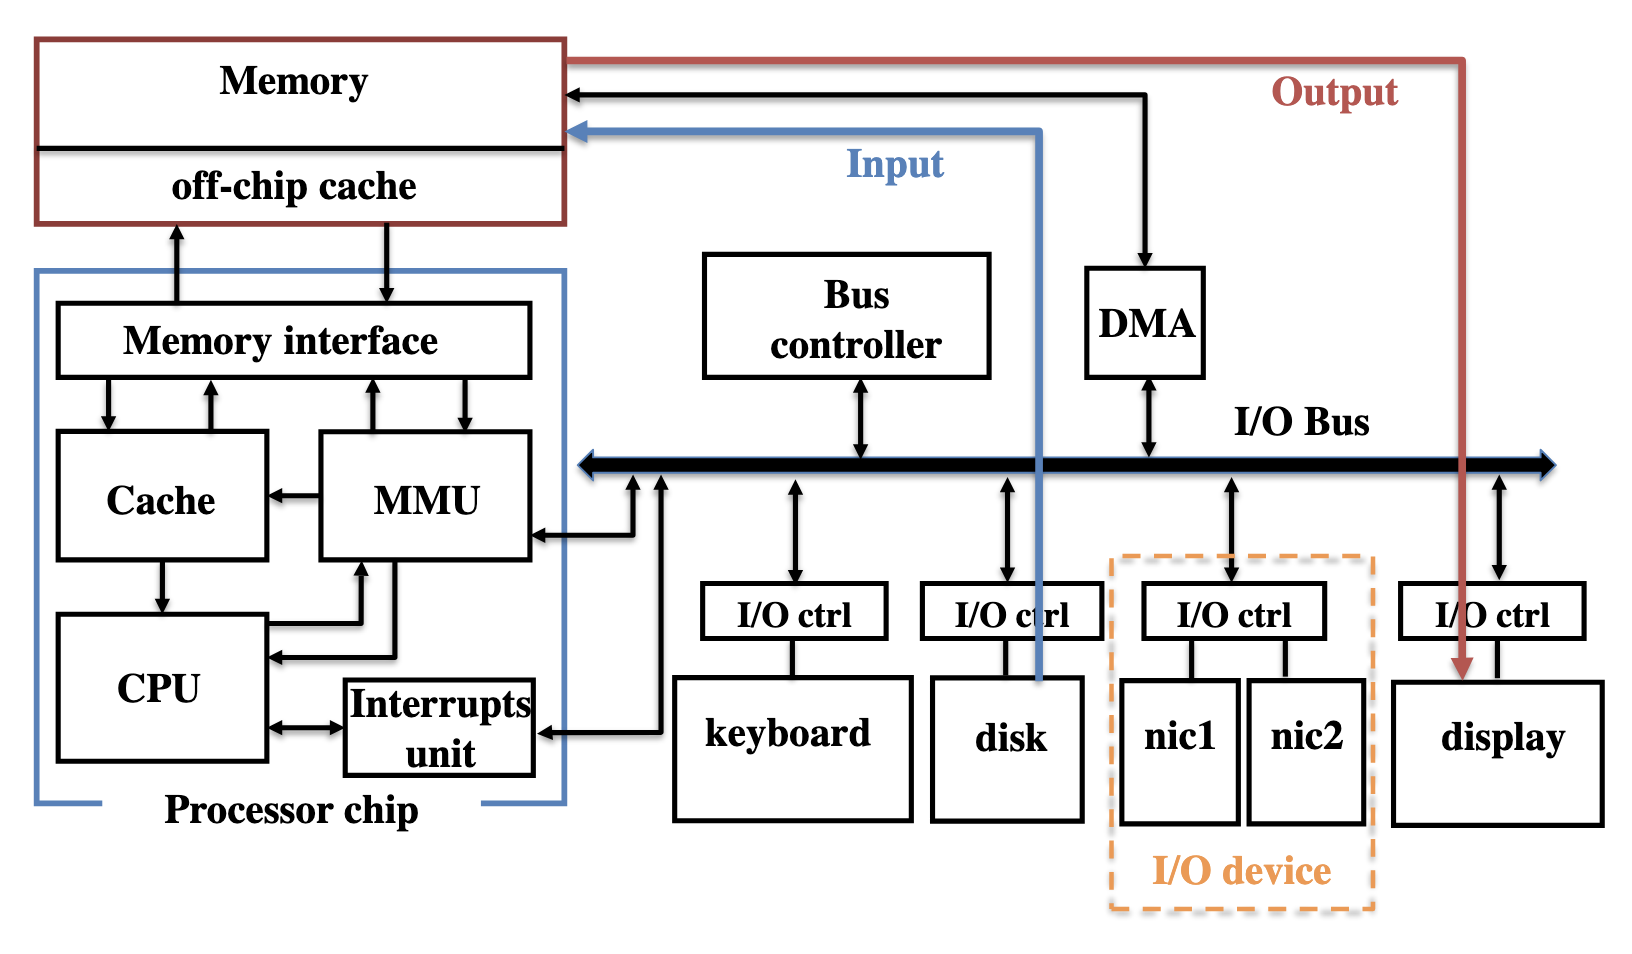
\includegraphics[width=13cm]{images/input-output-iodevice.png}
    \caption{Input/output e I/O devices}
\end{figure}

\hspace{-15pt}Solitamente le operazioni di I/O hanno un grosso impatto sul tempo di esecuzione dei programmi.
Supponiamo per esempio di andare a calcolare il tempo di esecuzione con \(T_{exe} = T_{cpu} + T_{I/O} = \frac{1}{10}T_{cpu}\) perciò
\(T_{exe} = \frac{11}{10}T_{cpu}\).\\\\
\hspace{-15pt}Se andiamo ad aumentare il tempo \(T_{cpu}\) di 10 volte lasciando inalterato il \(T_{I/O}\) abbiamo
un \(T_{cpu}^{enhanced} = \frac{1}{10} T_{cpu}\) così \(T_{exe} = \frac{1}{10}T_{cpu} + \frac{1}{10}T_{cpu} = \frac{1}{5}T_{cpu}\)
Consideriamo copi che l'aumento di velocià uguale a: \[\frac{T_{exe} \text{before enhancmente}}{T_{exe} \text{after enhancmente}} = \frac{11}{5} = 5.5\]

\subsection{Legge di Amdahl}
Proposto da Gene Amdahl nel 1967. Si occupa della potenziale velocità massima raggiungibile da un programma parallelo quando si aumenta il numero di processori da 1 a N.
Può essere applicato a qualsiasi processo di ottimizzazione. 
Si consideri un programma in cui solo la frazione f può essere ottimizzata (ad esempio, parallelizzata utilizzando N processori), mentre la frazione (1-f) rimane inalterata (ad esempio, è intrinsecamente sequenziale).
\[\text{Speedup} = \frac{\text{Tempo di esecuzione proma del miglioramento}}{\text{Tempo di esecuzione dopo il migliormaneto}} = \frac{T(1- f) + Tf}{T(1 - f) + \frac{Tf}{N}} = \frac{1}{(1 - f) + \frac{f}{N}}\]

\begin{observation}
    L'accelerazione è vincolata dalla frazione sequenziale (1-f), cioè dalla parte del processo che non posso (o non sono in grado) di valorizzare!
\end{observation}

\hspace{-15pt}
Le prestazioni del sottosistema I/O sono molto importanti, ma non sono tutto. Altri aspetti importanti sono:
\begin{itemize}
    \item \textbf{Affidabilità} gestite da metriche del tempo medio al guasto (MTTF), prevenzione dei guasti (componenti migliori), tolleranza ai guasti (introduzione di un certo livello di ridondanza).
    \item \textbf{Disponibilità} invece gestite da Tempo medio di riparazione (MTTR), e dalla formula \(\frac{MTTF}{MTTF + MTTR}\)
\end{itemize}

\hspace{-15pt}I dispositivi I/O hanno due tipologie di porte: porte di controllo, e porte data.
\begin{itemize}
    \item Controllo: sia comandi che rapporti di stato, come diciamo al dispositivo cosa fare, come il dispositivo ci racconta le sue caratteristiche, come il dispositivo ci informa sullo stato operativo.
    \item Data: Alla/dalla memoria del dispositivo.
\end{itemize}

\vspace{-10pt}
\begin{figure}[!h]
    \centering
    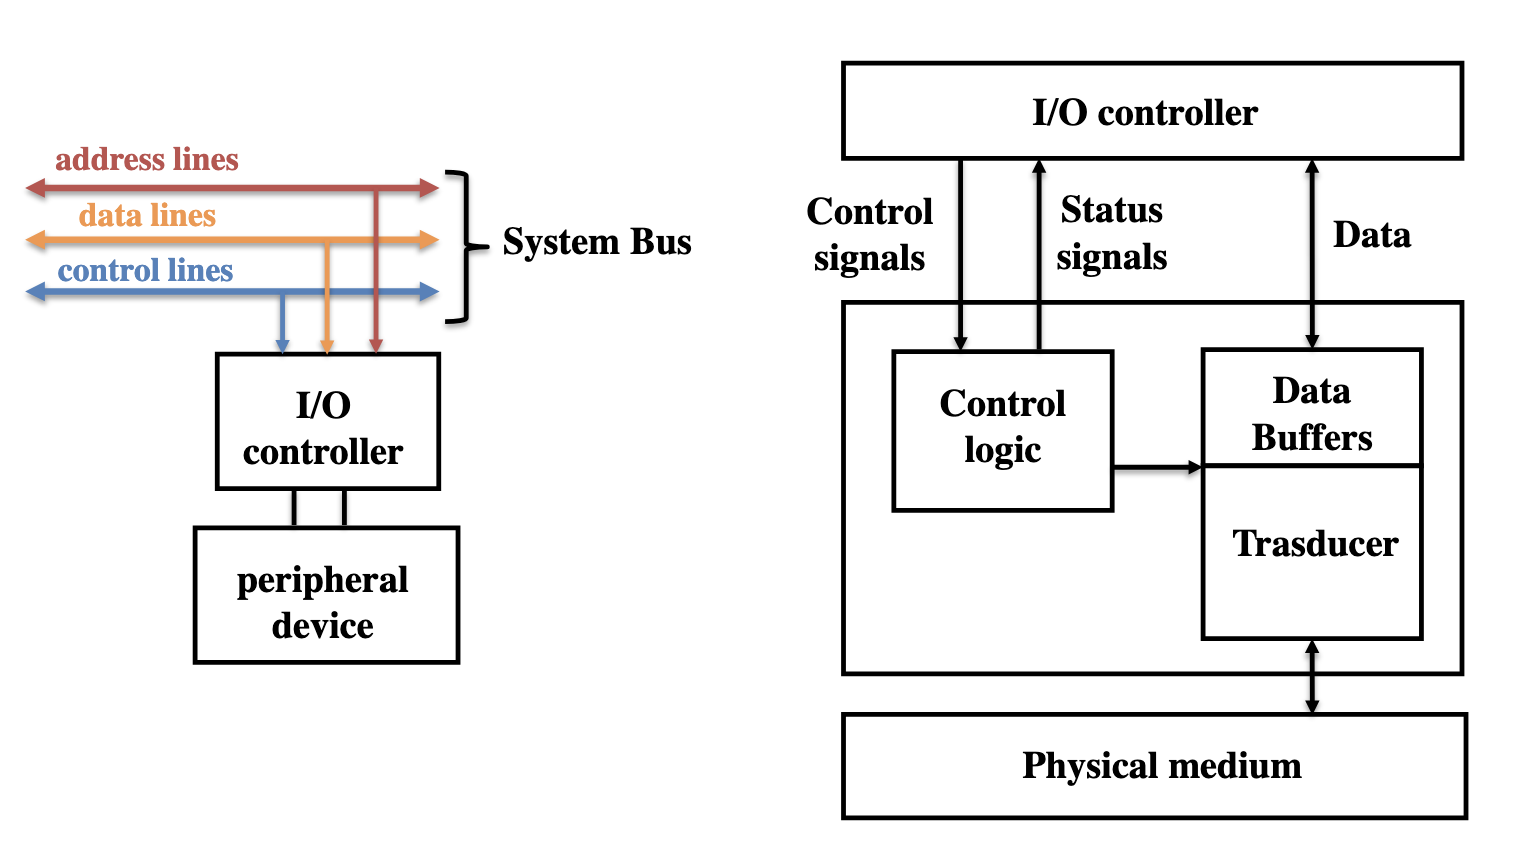
\includegraphics[width=12cm]{images/generic-io-device.png}
    \caption{I/O device generico}
\end{figure}

\hspace{-15pt}I/O funzioni di controllo abbiamo invece il control and imting, la comunicazioni fra processi (command decoding, data exchange, status reporting, address recognition), comunicazione
fra i device, il data buffering (per ottimizare il trasferimento dei dati e compensare le differenze di velocità).

\subsection{Connessione bus}
Servono per il controllo del trasferimento da un dispositivo al processore:
\begin{enumerate}
    \item la CPU controlla lo stato del dispositivo del modulo I/O.
    \item Il controller I/O restituisce lo stato se pronta.
    \item La CPU richiede il trasferimento dei dati tramite un comando al controllore.
    \item Il controller I/O riceve i dati dal dispositivo periferico.
    \item il controller I/O trasferisce i dati al processore.
\end{enumerate}

\begin{wrapfigure}{r}{7cm}
    \vspace{-35pt}
    \centering
    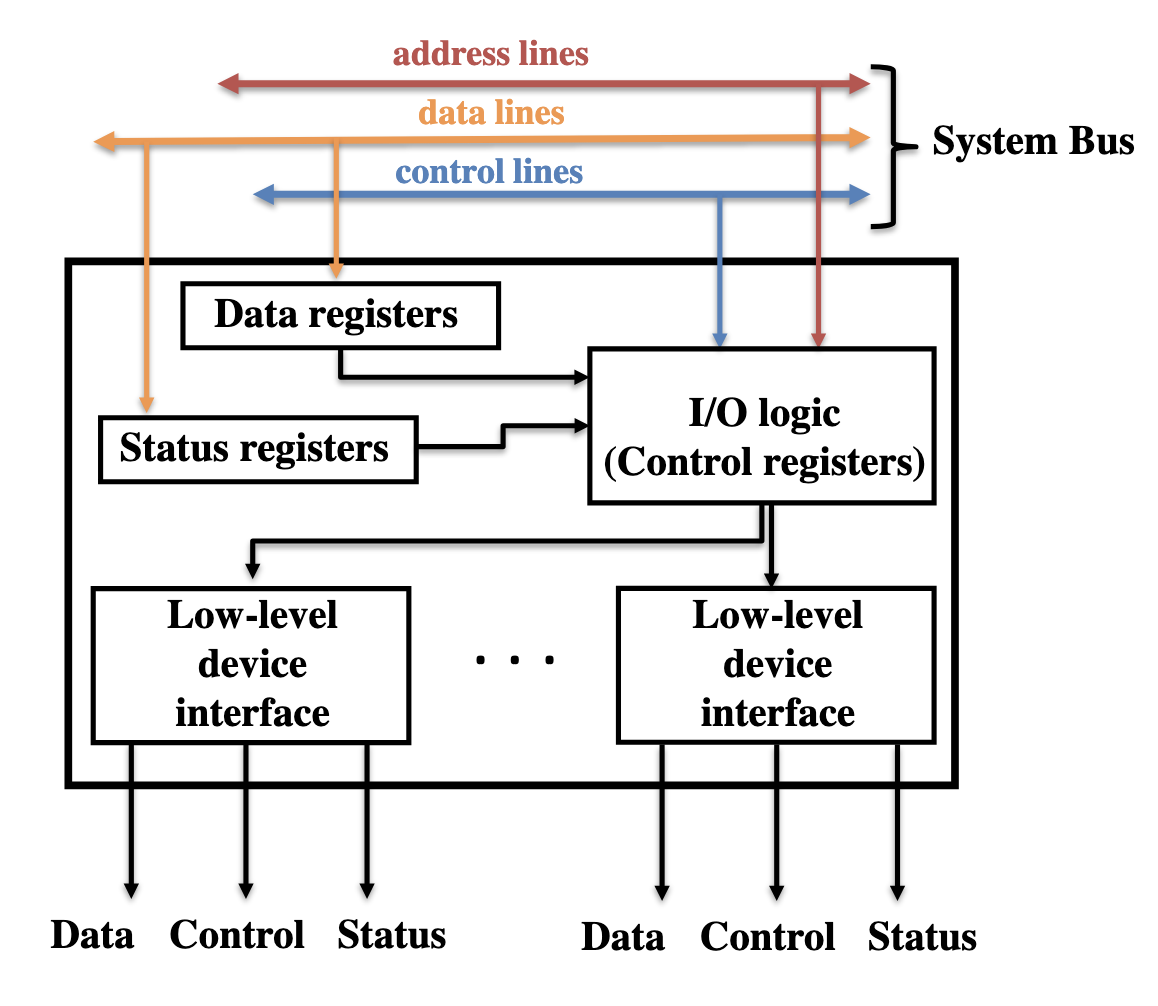
\includegraphics[width=6cm]{images/io-controller-diagram.png}
    \caption{I/O device generico}
\end{wrapfigure}
Questi passaggi richiedono una o più azioni di arbitrato del bus per implementare il protocollo di comunicazione.
Andiamo ora a definire l'interconnesione fra bus, essa si definisce come una raccolta di linee di dati trattate insieme come un singolo segnale logico
utilizzato anche per indicare una raccolta condivisa di linee con più dispositivi connessi (chiamati rubinetti), si definiscono su essi alcuni fattori di prestazione: lunghezza fisica, numero di prese collegate.
\\\\Un bus è un mezzo di trasmissione condiviso, solo un dispositivo alla volta può trasmettere con successo. Il bus di sistema collega i principali componenti (processore, memoria, bus I/O), centinaia di linee separate, linee classificate in tre gruppi: dati, indirizzo, controllo.
\newpage

% \begin{wrapfigure}{l}{2.5cm}
%     \centering
%     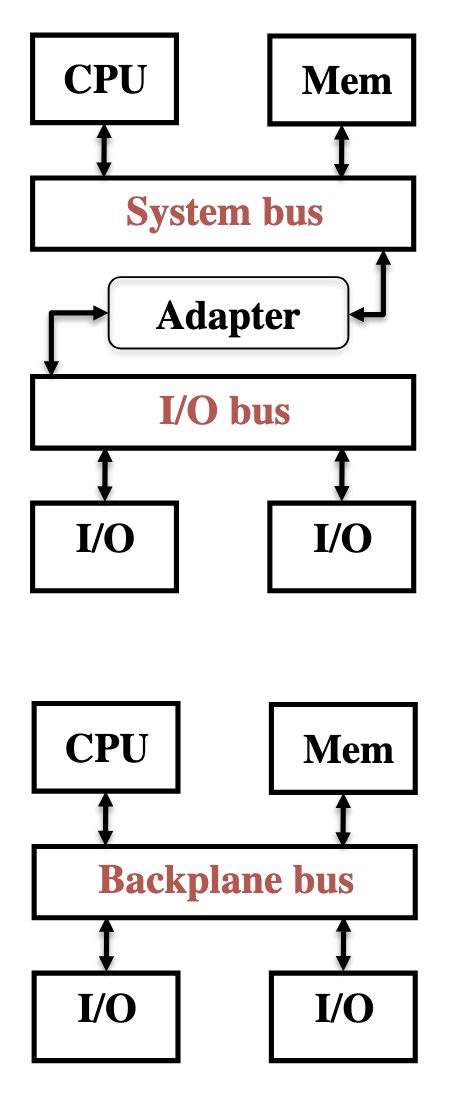
\includegraphics[width=2.5cm]{images/buses-type.png}
% \end{wrapfigure}
\hspace{-15pt}Alcuni tipi di bus sono:
\begin{itemize}
    \item \textbf{System bus} Collega processore e memoria, I/O interfacciato con adattatori: breve, pochi tocchi e quindi più veloce e larghezza di banda elevata, inoltre non è standard (ovvero specifico del sistema).
    \item \textbf{I/O bus} Connette dispositivi I/O, nessuna connessione diretta con processore e memoria: più tempo, più tocchi è uguale a più lentezza e larghezza di banda inferiore. E' uno standard di settore (ad es. ATA/SCSI).
    \item \textbf{Backplane bus} Connette CPU, memoria, dispositivi I/O. Lunghe, molti tocchi allora lento e larghezza di banda medio/bassa. Gestisce diversi dispositivi con diverse larghezze di banda ed è standard di settore.
\end{itemize}

\subsubsection{Bus design}
Il design di un bus si basa su soddisfare gli obbiettivi di avere un alta performance, standardizzazione e bassi costi. Per esempio 
il bus di sistema enfatizza le prestazioni, l'I/O e i bus backplain enfatizzano i costi e la standardizzazione.\\
Uno dei problemi principali di progettazioni da affrontare è il seguente: 
\begin{itemize}
    \item I cavi sono condivisi o separati? La risposta è che i bus più ampi (ovvero, una maggiore larghezza di banda) sono più costosi e più suscettibili allo skew.
    \item Come viene acquisito e rilasciato il controllo del bus? La riposta è tramite due metodologie \textbf{Atomic transactions} che permette una bassa utilizzazione ed una bassa complessita, e le \textbf{Split-transactions}
    dove le richieste/risposte possono essere intervallate; ciò significa un utilizzo più elevato ma un design più complesso (ad es. ID per identificare richieste diverse).
    \item Il bus ha è cloccato (ha un tempo di clock)? Per rispondere al problema del clock bisogna introdurre due opzioni possibili.
    \begin{itemize}
        \item \underline{\textbf{Sincrono}}. Tutti i dispositivi collegati al bus condividono lo stesso bus clock. Gli eventi si verificano all'estremità del segnale di clock. Un protocollo possibile è che al ciclo \(X\) l'unità di I/O scrive una richiesta READ sul bus; al ciclo \(X + \Delta\) l'unità può leggere i dati dal bus.
        \(\Delta\) è il tempo massimo per scrivere i dati sul bus da parte di un'unità collegata.\\
        Potenziale abbiamo il problema di skew dell'orologio e questa soluzione è limitata a bus brevi (ad esempio, bus di sistema).
        \item \underline{\textbf{Asincrono}}. Il bus non ha il clock. Nessun disallineamento dell'orologio, si occupa di dispositivi con velocità diverse: può essere più lungo, quindi più lento. \\
        Richiede protocolli di handshaking. Inoltre il protocollo possibilo funzione nel seguente modo (3 linee di controllo, 1 linea dati in cui i dati e l'indirizzo sono multiplexati): UIO1 scrive una richiesta READ (WRITE) ReadReq (WriteReq) nella linea di controllo e 
        l'indirizzo nella linea dati, UIO2 legge il indirizzo e scrive un ACK nella linea di controllo a UIO13. UIO2 scrive i dati sul bus e scrive la riga DataReadycontrol per notificare UIO14. UIO1 legge i dati e invia un ACK nella linea di controllo a UIO2.
    \end{itemize}
    \item Come si devide chi prende un bus per trasferire dati? Le comunicazioni bus devono essere gestite da un protocollo di comunicazione. Ne possiamo vedere due:
    \begin{itemize}
        \item \underline{\textbf{Bus master}}. Il concetto dietro questo protocolle è che, un unità che può avviare una richiesta di bus. Esso ha una configurazione più semplice: un solo master mentre di solito i bus hanno più master.
        \item \underline{\textbf{Arbitration}}. Il concetto invece di questo protocolle è che si va ha scegliere un master tra più richieste cercando di implementare la priorità e l'equità (prevenendo la fame). Solo un master alla volta (tutti gli altri ascoltano il bus). Il ruolo dell'arbitro è gestire le richieste del bus e assegnare le sovvenzioni considerando le priorità e l'equità.\\\\
        Per andare ad implementale questo sistema possiamo usare un metodo \textbf{centralizzato}, dove un dispositivo dedicato (Arbiter) raccoglie le richieste e poi decide (potenziale problema di collo di bottiglia). Si può usare un metodo ri raccolta Daisy-chain, non equo, oppure con linee di richiesta/risposta indipendenti (ampiamente utilizzate).
        \\\\Oppure possiamo usare un metodo \textbf{distribuito} dove ogni dispositivo vede le richieste contemporaneamente e partecipa alla selezione del master successivo (più complesso da realizzare e necessita di molte linee di controllo).
    \end{itemize}
\end{itemize}


\subsection{Gestione dell I/O}
Quando andiamo a parlare di gestione dei dispositivi di input output ci chiedimao come la CPU da i comandi 
hai dispositivi di I/O? Come la CPU sa quando i dispositivi di I/O completando le operazioni? Come fanno i 
disponsitivi di I/O ad eseguire il data transfers?\\\\
Partiamo dal rispondere alla prima domanda. Inanzitutto soltato il sistema operativo può mandare comandi hai dispositiv
di I/O ed i programmatori per mandare comandi all'I/O deve utilizzare delle chiamate di sistema. Da qui possiamo avere
due opzioni per mandare comandi hia device di I/O:
\begin{itemize}
    \item I/O istruzioni: istruzioni ISA che indirizzano i registri dei dispositivi I/O. Sono delle istruzioni di privilegio disponibile soltato in kernel mode.
    \item Memory-mapped I/O: una porzione degli indirizzi fisici rispervata all'I/O.
\end{itemize}

\hspace{-15pt}

\subsection{Memory-mapped I/O}
I registri interni dei dispositivi sono mappati su locazioni di memoria principali (a indirizzi fisici riservati). 
I comandi di I/O sono lettura/scrittura di memoria standard. Le operazioni in quelle posizioni vengono reindirizzate ai controller del dispositivo dalla MMU. 
Gli accessi in modalità utente alle aree mappate in memoria generano eccezioni di violazione della memoria.

\subsection{Programmed I/O}
Per andare invece ora a rispondere alla seconda domanda che era stata posta. Come la CPU sa quando i dispositivi di I/O completando le operazioni?
Introduciamo due concetti che possano risolvere questo probelma:
\begin{itemize}
    \item Programmed I/O: la cpu gestisce direttamente le operazioni e gli status di I/O.
    \item Interrupt-driven I/O: Un interrupt è un evento asincrono proveniente da un dispositivo (ad es. modulo I/O, timer, controller DMA). A volte le eccezioni sono anche c
    hiamate interruzioni (o comprendono interruzioni). In generale, le eccezioni sono eventi sincroni che interrompono l'esecuzione del programma (ad esempio, overflow aritmetico, istruzione non definita).
\end{itemize}

\hspace{-15pt}Nel caso specifico del programmed I/O come scritto sopra la CPU ha un diretto controllo sopra l'I/O, quindi 
gestisce lo stato di rilevamento, i comandi di lettura e scrittura ed il trasferimento dei dati. Con questo sistema i ll dispositivo I/O ha un ruolo passivo e 
la CPU attende che il modulo I/O completi le operazioni (polling). \\\\
Nel pulling il processore interroga il registro di stato del dispositivo I/O. Esso ha come pro una facile implmentazione
mentre come contro una perdita di cicli del processore perchè la CPU è molto più veloce che i dispositivi di I/O. La cpu deve leggere lo sato dei registri
molte volte solo per scoprire che il dispositivo non ha completato l'operazione.

\subsection{Interrupt-driven I/O}
Il problema principale visto nel programmed I/O è la perdita di tempo per l'alta velocità della CPU, come alternativa al polling
si introduce quello che viene chiamato interrupts.
\begin{itemize}
    \item La CPU invia comandi a un dispositivo e continua a svolgere altre attività. 
    \item Il dispositivo I/O genera un interrupt quando lo stato cambia, cioè i dati sono pronti.
    \item Gli interrupt di I/O sono asincroni.
    \item I/O interrupts sono prioritari, dove in particolare i dispositivi I/O con larghezza di banda elevata hanno una priorità maggiore rispetto a quelli con larghezza di banda ridotta.
\end{itemize} 

\hspace{-15pt}Dal punto di vista della CPU viene inviato un comando I/O (ad esempio, un carico mappato in memoria), nel fra tempo viene fatto altro lavoro, viene poi controllato l'interrupt alla fine del ciclo fetch-execute
e se l'iterrupt viene ricevuto salva il contesto corrente (ovvero i registri, non necessariamente tutti) e passa al livello privilegiato (ovvero PL1 su processore ARM), sulla base dell'ID dell'interrupt e della priorità dell'interrupt, il gestore dell'interrupt associato è pronto per essere eseguito, \footnote{I passaggi precedenti sono atomici dal punto di vista del sistema operativo!} 
esegui poi il gestore (ovvero, il sistema operativo gestisce l'interrupt) e ripristina il contesto per l'esecuzione dell'istruzione successiva: \footnote{il ripristino è un'operazione atomica per il sistema operativo! }

\begin{example}
    Facciamo ora un esempio, assumiamo di avere una CPU ad una velocità di 500MHz ed un costo di polling di 400 cicli. Abbiamo poi un mouse come dispositivo a banda lenta.
    Vogliamo aver un poll di 30 volte al secondo.\\\\
    Per calcolare i cicli al secondo per polling scriviamo (30 poll/s) * 400 = 120000 cycles/s, e la percentuale di cicli spesi
    per polling si calocla fancendo 12K/500M = 0.002\(\%\). Abbiamo dunque un overhead accettabile.\\\\
    Prendiamo ora un disco (che è un dispositivo ad alta lunghezza si banda) che ha 4MB/s di transfer rate e 16B interface.\\
    Per non mancare i dati dobbiamo eseguire il poll abbastanza spesso, quindi (4MB/s)/16B = 250 K/s, vista come percentuale di cicli
    abbiamo 100M / 500 M = 20\(\%\), questo risultato non è accetabile perchè Abbiamo speso il 20\(\%\) dei cicli solo per controllare i registri I/O, non per il trasferimento dei dati
\end{example}

\subsection{Data transfers (DMA)}
Andiamo ora a rispondere all'ultima domanda che ci eravamo posti, come i device di I/O eseguno il trasferimento dei dati?
Sappiamo ora che l'I/O guidato da interrupt elimina i problemi di polling, tuttavia, il sistema operativo deve trasferire i dati una parola alla volta. Questo va bene solo per dispositivi I/O a bassa larghezza di banda (ad es. mouse), per ovviare
a questo problma introduciamo la direct memory access (DMA).\\\\
Esso è meccanismi che forniscono a un dispositivo di controllo I/O la capacità di trasferire i dati direttamente da e verso la memoria principale senza coinvolgere la CPU. 
DMA disaccoppia il protocollo CPU-memoria dal protocollo memoria-dispositivo I/O. Interrupt utilizzati dal dispositivo I/O per comunicare con la CPU solo al completamento del trasferimento I/O o quando si verifica un errore.\\\\
DMA è implementato con un controller specializzato. Per eseguire DMA, un dispositivo I/O è collegato a un controller DMA: è possibile collegare più dispositivi allo stesso controller. Il controller stesso è visto come un dispositivo I/O mappato in memoria, 
inoltre il controller DMA si occupa dell'arbitrato del bus e del trasferimento dei dati: diventa il master del bus. Il controller DMA e la CPU si contendono il bus di memoria.
Ci sono tre passi nel transfer DMA:
\begin{enumerate}
    \item La CPU imposta DMA fornendo identità, op, indirizzo di memoria e numero di byte da trasferire.
    \item DMA avvia l'operazione sul dispositivo e arbitra la connessione. Trasferisce i dati dal dispositivo o dalla memoria.
    \item Una volta completato il trasferimento DMA, il controller invia un interrupt alla CPU.
\end{enumerate}

\begin{example}
    Facciamo un esempio, assumiamo i seguenti dati: 500Mhz CPU, il device di un disco ha un tempo di trasferimento 4MB/s, 16B di interfaccie
    e un utilizzo di 50\(\%\), la gestione degli interrupt richiede 400 cicli, il trasferimento dei dati richiede 100 cicli, l'installazione DMA richiede 1600 cicli, trasferisce un blocco da 16 KB alla volta.\\\\
    Overhead del processore per I/O guidato da interrupt senza DMA (il processore è coinvolto per ogni trasferimento di dati (16 B)) si calcola facendo 0.5 * (4MB/s) / (16B) * [(400 + 100) cicli / 500M cicli/s] = 12.5 \(\%\).\\\\
    Overhead del processore per I/O guidato da interrupt con trasferimento DMA (Il processore è coinvolto una volta per trasferimento a blocchi (16 KB)) si calcola invece facendo 0.5 * (4M B/s) / (16KB) * [(1600 + 400) / (5ooM cicli/s)] = 0.05 \(\%\)
\end{example}

\hspace{-15pt}Notiamo da questo esempio che Senza DMA: il processore avvia tutti i trasferimenti di dati, tutti i trasferimenti passano attraverso la traduzione degli indirizzi (MMU), i trasferimenti possono essere di qualsiasi dimensione e attraversare i limiti della pagina virtuale, 
nessun impatto sulla gerarchia della cache, le cache non contengono mai dati obsoleti.\\\\
Mentre con DMA: il controller DMA avvia i trasferimenti di dati, esiste un altro percorso per il sistema di memoria, potenziali problemi: 
i controller DMA utilizzano indirizzi virtuali o fisici? Cosa succede se scrivono i dati in una posizione di memoria cache?\\\\
Per rispondere alla domanda, quali indirizzi il processore specifica al controller DMA? Abbiamo la virtual DMA e la 
DMA fisica:
\begin{itemize}
    \item Virtual DMA: Il controller DMA deve eseguire internamente la traduzione degli indirizzi utilizzando una piccola cache (TLB) inizializzata dal sistema operativo quando richiede un trasferimento I/O. Complesso ma flessibile (ad esempio, grandi trasferimenti tra pagine).
    \item Physical DMA: Il controller DMA funziona con indirizzi fisici. Trasferimenti alla granularità della pagina, il sistema operativo suddivide i trasferimenti di grandi dimensioni in blocchi delle dimensioni della pagina. Più semplice, ma meno flessibile.
\end{itemize}

\hspace{-15pt}La DMA ha anche un'integrazione con la cache essendo che la memorizzazione nella cache riduce le istruzioni della CPU e la latenza di accesso ai dati e riduce l'utilizzo della memoria da parte della CPU, lasciando così più larghezza di banda di memoria/bus per i trasferimenti DMA. Ma le cache introducono un problema di coerenza per DMA: se il DMA scrive nella memoria principale, la versione dei dati nella cache è obsoleta. Per le cache write-back, il controller DMA potrebbe leggere i vecchi valori dei dati dalla memoria mentre i dati nella cache hanno il set di bit sporchi. La soluzione è lo svuotamento/invalidamento selettivo delle linee memorizzate nella cache 
coinvolte nei trasferimenti DMA: richiede una logica aggiuntiva per la coerenza della cache HW!\\\\
L'accesso hai device è gestito tramite, uno stack software che fornisce modi per accedere a un'ampia gamma di dispositivi I/O. 
Un'interfaccia comune, in POSIX equivalente all'accesso ai file, in termini di chiamate di sistema 
di apertura/chiusura, lettura/scrittura. Driver di dispositivo per ogni dispositivo specifico, parte superiore HW, 
indipendenti (per migliorare la portabilità), parte inferiore HW-dipendente



% !TeX spellcheck = it_IT
\newpage
\section{Dischi rigidi}
Alcuni tipi di storage device sono per esempio i dischi magnetici e le flash memory.

\begin{definition}[Dischi magnetici]
    I dischi magnetici è un tipo di archiviazione che raramente viene danneggiata. 
    Grande capacità a basso costo. Accesso casuale a livello di blocco. 
    Prestazioni lente per l'accesso casuale. Migliori prestazioni per l'accesso in streaming.
\end{definition}

\begin{definition}[Flash memory]
    Archiviazione che raramente viene danneggiata. Buona capacità a costo intermedio (2 \(\times\) disco). 
    Accesso casuale a livello di blocco. Buone prestazioni per le letture; peggio per le scritture casuali.
\end{definition}

\subsection{Dischi magnetici}
I dischi magnetici hanno circa 1 micron di larghezza, lunghezza d'onda della luce è di circa 0.5 micron, 
risoluzione dell'occhio umano: 50 micron, 100K su un tipico disco da 2,5 pollici. Separato da regioni 
di guardia inutilizzate, riduce la probabilità che le tracce vicine vengano danneggiate durante le scritture 
(ancora una piccola possibilità diversa da zero). \\\\
La lunghezza della traccia varia a seconda del disco, all'esterno: più settori per traccia, maggiore larghezza di banda, il disco è organizzato in regioni di tracce 
con lo stesso numero di settori/traccia, viene utilizzata solo la metà esterna del raggio. La maggior parte
dell'area del disco nelle regioni esterne del disco

\subsubsection{Settore}
I settori contengono sofisticati codici di correzione degli errori, il magnete della testina del disco ha un campo più ampio della traccia, nasconde le corruzioni dovute alle scritture di tracce vicine
\begin{itemize}
    \item \textbf{Sector sparing}. Rimappa i settori danneggiati in modo trasparente ai settori di riserva sulla stessa superficie.
    \item \textbf{Slip sparing}. Rimappa tutti i settori (quando c'è un settore danneggiato) per preservare il comportamento sequenziale.
    \item \textbf{Track skewing}. Numeri di settore spostati da una traccia all'altra, per consentire il movimento della testina del disco per operazioni sequenziali.
\end{itemize}

\hspace{-15pt}A basso livello il controller accede ai singoli settori. La dimensione tipica del settore è di 256/512 byte. 
Identificato da una tripla: \(<\)\#cilindro, \#faccia, \#settore\(>\).\\\\
Al livello superiore, il driver del disco raggruppa un insieme di settori contigui in un blocco. La dimensione tipica del blocco è di 2/4/8 Kbyte, 
identificata da un puntatore su uno spazio di indirizzi contiguo (da 0 a max-blocks).\\
Dato un numero di sector \(b\), ed una tripla \(<c,f,s>\) abbiamo che.
\[b = c(\text{\#faces} \cdot \text{\#sectors}) + f(\text{\#sectors}) + s\]
\#faces sono il numero di facce in un disco mentre \#sectors sono il numero di settori per track. Di conseguenza a questa formula
abbiamo che:
\[c = b \:\: div \:\: (\text{\#faces} \cdot \text{\#sectors}) \hspace{18pt} f = (b \:\: div \:\: (\text{\#faces} \cdot \text{\#sectors}))div \:\: \text{\#sectors}\]
\[s = (b \:\: div \:\: (\text{\#faces} \cdot \text{\#sectors}))mod \:\: \text{\#sectors}\]

\begin{example}
    Disco con 100 cilindri, 4 facce, 2000 settori per traccia. Un file utilizza i blocchi 94421, 94422, 94423. Qual è il \(<c,f,s>\) per ogni blocco?
    Possiamo calcolare facendo:\\ \(c = 94421 \:\: div \:\: (4 \cdot 2000) = 1\) (rimangono 6421). \(f = 6421 \:\: div \:\: 2000 = 3\) (rimangono 421) quindi \(s = 421\).
    Pertanto le triple sono: \(<11, 2, 421>, <11, 3, 422>, <11, 3, 423>\).
\end{example}

\subsubsection{Disk performance}
Fra i puinti principali nel calcolo delle performance di un disco è la sua latenza. Per calcolare la disk latency:
\[\text{Disk latency = Seek time + Rotation time + Transfer Time}\]

\hspace{-15pt}In questa formula possiamo notare 3 componenti:
\begin{itemize}
    \item \textbf{Seek time}. Tempo per spostare il braccio del disco sulla traccia (1-20ms). Regolazione fine della posizione necessaria affinché la testina si "assesti". Tempo di cambio testina ~ tempo di cambio traccia (su dischi moderni).
    \item \textbf{Rotation time}. Tempo di attesa per la rotazione del disco sotto la testina del disco Rotazione del disco: 4, 15 ms (a seconda del prezzo del disco).
    \item \textbf{Transfer time}. Tempo di trasferimento dei dati su/fuori dal disco Velocità di trasferimento testina disco: 50-100 MB/s (5-10 usec/settore). Velocità di trasferimento host dipendente dal connettore I/O (USB, SATA, ...).
\end{itemize}

\begin{example}
    Quanto ci vuole per completare 500 letture casuali del disco, in ordine FIFO? Ricerca: media 10,5 msec. Rotazione: media 4,15 msec. Trasferimento: 5-10 usec. 500 * (10,5 + 4,15 + 0,01)/1000 = 7,3 secondi.
\end{example}

\begin{example}
    Quanto tempo occorre per completare 500 letture sequenziali del disco? Tempo di ricerca: 10,5 ms (per raggiungere il primo settore). Tempo di rotazione: 4,15 ms (per raggiungere il primo settore). Tempo di trasferimento: (traccia esterna) 500 settori * 512 byte / 128 MB/sec = 2 ms Totale: 10,5 + 4,15 + 2 = 16,7 ms. \\
    Potrebbe essere necessaria una testina aggiuntiva o un interruttore di traccia (+1ms). Il buffer di traccia può consentire la lettura fuori servizio di alcuni settori dal disco (-2ms)
\end{example}


\begin{example}
    Disco con 100 cilindri, 4 facce, 2000 settori per traccia. Un file usa i blocchi 94421, 94422, 94423 \((<11,3,421> <11,3,422> <11,3,423>)\). 
    \\Un settore viene letto in 0,01 ms, il tempo di ricerca tra due tracce consecutive è di 0,01 ms e il tempo medio per raggiungere il settore desiderato è la metà del tempo di rotazione. 
    \\Considerando che il braccio è al cilindro 22 e che il controller DMA ha abbastanza buffer, calcola il tempo per leggere i blocchi di file.(22-11)*0.01 + 20/2 + 3*0.01 = 10.14ms
\end{example}

\subsection{Dishi SSD}
Un Solid StateDrive (SSD) è un dispositivo di archiviazione non volatile basato sulla tecnologia di memoria flash. Gli SSD sono più affidabili e più veloci dei dischi rigidi (HD) perché non hanno parti mobili e nessun tempo di ricerca, sli SSD usano comunemente una semplice pianificazione FCFS policy. 
Consumano meno energia e sono più costosi per MB di dati. La capacità dell'HD è in genere maggiore. In alcuni sistemi, gli SSD vengono utilizzati come ulteriore livello di cache nella gerarchia della memoria.
\\\\
All'interno delle flash memory abbiamo che le scritture devono essere per "pulire" le celle; nessun aggiornamento in atto. Cancellazione di blocchi di grandi dimensioni richiesta prima della scrittura.
Blocco di cancellazione fra 128 ed i 512 KB. Tempo di cancellazione: diversi millisecondi, scrittura/lettura pagina (2-4 KB) in circa 50-100 usec.

\subsubsection{Flash translation layer}
Per evitare il costo di una cancellazione per ogni scrittura, le pagine vengono cancellate in anticipo. Pagine pulite sempre disponibili per una nuova scrittura, questo significa che una scrittura non può essere indirizzata ad una pagina arbitraria in memoria, ma solo ad una pagina precedentemente cancellata, cosa succede se si riscrive un blocco di un file? La pagina che contiene il blocco non può da riscrivere subito...
Deve essere prima cancellato ma con le pagine circostanti!
Viene utilizzata una pagina pulita per applicare la scrittura, ma questa pagina è da qualche parte nel disco...
La vecchia pagina va nella spazzatura per il riciclaggio. Come sapere dove sono le pagine del mio file?\\
Il firmware del dispositivo flash associa la pagina logica \# a una posizione fisica: sposta le pagine live 
secondo necessità per la cancellazione. Garbage collect blocco di cancellazione vuoto copiando le pagine 
live in una nuova posizione, abbiamo dunque livellamento dell'usura. 
Puoi scrivere ogni pagina fisica solo un numero limitato di volte: evita le pagine che non funzionano più. 
Trasparente per l'utente del dispositivo.

\subsubsection{File system flash}
I file system sui dischi magnetici non hanno bisogno di dire al disco quali blocchi sono in uso: 
quando un blocco non è più utilizzato viene contrassegnato come libero nella bitmap, il file system 
lo riutilizza quando vuole. Quando questi FS sono stati utilizzati per la prima volta su unità flash, 
le prestazioni sono diminuite drasticamente nel tempo.\\\\
Il Flash Translation Layer si è dato da fare con la garbage collection: i blocchi live devono essere 
rimappati in una nuova posizione, per compattare le pagine libere per poter procedere con la cancellazione dei blocchi. 
Questo anche con una grande quantità di spazio libero, ad esempio, se FS sposta un file di grandi dimensioni da un 
intervallo di blocchi a un altro, lo storage non sa che i vecchi blocchi possono andare nella spazzatura, a meno che FS 
non lo dica!\\\\
Comando TRIM: il file system indica al dispositivo quando le pagine non sono più in uso. Aiuta il livello di traduzione dei file a ottimizzare la raccolta dei rifiuti. Introdotto tra il 2009 e il 2011 nella maggior parte dei sistemi operativi.



\newpage
\section{Introduzione ai sistemi operativi}
Inanzitutto iniziamo con una Definizione del sistema operativo: software per gestire le risorse di un computer per i suoi utenti e applicazioni. 
Sfide del sistema operativo: affidabilità, sicurezza, reattività, portabilità, ... storia del sistema operativo: a che punto siamo?
\\\\Andiamo ora a rispondere alla domanda, cos'è un sistema operativo?\\
E' software per gestire le risorse di un computer per i suoi utenti e applicazioni- Funzionalità principali: pianificazione delle risorse, memoria virtuale, comunicazione tra processi (IPC) 
e meccanismi di sincronizzazione.

\subsection{Ruoli del sistema operativo}
Abbiamo una serie di ruoli che un sistema operativo va a prendere, essi sono:
\begin{itemize}
    \item \textbf{Referee}: Allocazione delle risorse tra utenti, applicazioni, isolamento di diversi utenti, applicazioni tra loro, comunicazione tra utenti, applicazioni.
    \item \textbf{Illusionist}: Ogni applicazione sembra avere l'intera macchina tutta per sé, numero infinito di processori, quantità (quasi) infinita di memoria, archiviazione affidabile, trasporto di rete affidabile.
    \item \textbf{Glue}: Fornisce servizi comuni e standard alle applicazioni, semplifica lo sviluppo di applicazioni, librerie, widget dell'interfaccia utente, ...
\end{itemize}

\begin{example}
    Prendiamo per esempio il file system. Abbiamo che:
    \begin{itemize}
        \item Referee: Impedisci agli utenti di accedere ai file degli altri senza autorizzazione, anche dopo che un file è stato eliminato e il suo spazio è stato riutilizzato.
        \item Illusionist: I file possono diventare (quasi) arbitrariamente grandi, i file persistono anche quando la macchina va in crash nel bel mezzo di un salvataggio.
        \item Glue: Directory con nome, printf, ...
    \end{itemize}
\end{example}
\end{document}
